% Este documento destina-se a servir como modelo para a produção de documentos
% de pesquisa do PPGINF/UFPR, como projetos, dissertações e teses. A classe de
% documento se chama "ppginf" (arquivo ppginf.cls) e define o formato básico do
% documento. O texto está organizado em capítulos que são colocados em
% subdiretórios separados. São definidos exemplos para a inclusão de figuras,
% códigos-fonte e a definição de tabelas.
%
% Produzido por Carlos Maziero (maziero@inf.ufpr.br) em Outubro de 2015.
% Adaptado de um modelo anterior construído pelo autor para o PPGIA/PUCPR.

% Opções da classe ppginf:
%
% - defesa  : versão para entregar à banca; tem espaçamento 1,5
%             e omite algumas páginas iniciais (agradecimentos, etc)
% - final   : versão pós-defesa, para enviar à biblioteca;
%             tem espaçamento simples e todas as páginas iniciais.
% - oneside : para impressão somente frente; use quando for gerar
%             somente o PDF, sem impressão.
% - twoside : para impressão frente/verso; use quando for gerar
%             uma versão impressa, para economizar papel.
% - ... (demais opções aceitas pela classe "book")

% Opções default: defesa, oneside
\documentclass[defesa,oneside]{ppginf}	% versão para a defesa
%\documentclass[final,oneside]{ppginf}	% versão final, só em PDF
%\documentclass[final,twoside]{ppginf}	% versão final, em PDF + impresso

% configurações de diversos pacotes, inclusive o fonte principal do texto
% Pacotes usados neste documento e suas respectivas configurações

% ------------------------------------------------------------------------------

% seleção de línguas do texto (a última é a principal/default)
\usepackage[english,brazilian]{babel}
\selectlanguage{brazilian}

% EXIGÊNCIA DA BIB@UFPR
% muda o título das referências para "Referências"
\addto{\captionsbrazilian}{\renewcommand{\bibname}{Refer\^encias}}

% ------------------------------------------------------------------------------
% Definição de fontes

% formato dos arquivos-fonte (utf8 no Linux e latin1 no Windows)
\usepackage[utf8]{inputenc}	% arquivos LaTeX em Unicode (UTF8)

% usar codificação T1 para ter caracteres acentuados corretos no PDF
\usepackage[T1]{fontenc}

% fonte usada no corpo do texto (descomente apenas uma)
\usepackage{newtxtext,newtxmath}	% Times (se não tiver, use mathptmx)
%\usepackage{lmodern}			% Computer Modern (fonte clássico LaTeX)
%\usepackage{kpfonts}			% Kepler/Palatino (idem, use mathpazo)
%\renewcommand{\familydefault}{\sfdefault} % Arial/Helvética (leia abaixo)

% A biblioteca central da UFPR recomenda usar Arial, seguindo a recomendação da
% ABNT. Essa é uma escolha ruim, pois fontes sans-serif são geralmente inade-
% quados para textos longos e impressos, sendo melhores para páginas Web.
% http://www.webdesignerdepot.com/2013/03/serif-vs-sans-the-final-battle/.

% fontes usadas em ambientes específicos
\usepackage[scaled=0.9]{helvet}		% Sans Serif
\usepackage{courier}			% Verbatim, Listings, etc

% ------------------------------------------------------------------------------

% inclusão de figuras
\usepackage{graphicx}			% incluir figuras em PDF, PNG, PS, EPS

% subfiguras (subfigure is deprecated, don't use it)
\usepackage[labelformat=simple]{subcaption}
\renewcommand\thesubfigure{(\alph{subfigure})}

% ------------------------------------------------------------------------------

% inclusão/formatação de código-fonte (programas)
\usepackage{listings}
\lstset{language=c}
\lstset{basicstyle=\ttfamily\footnotesize,commentstyle=\textit,stringstyle=\ttfamily}
\lstset{showspaces=false,showtabs=false,showstringspaces=false}
\lstset{numbers=left,stepnumber=1,numberstyle=\tiny}
\lstset{columns=flexible,mathescape=true}
\lstset{frame=single}
\lstset{inputencoding=utf8,extendedchars=true}
\lstset{literate={á}{{\'a}}1  {ã}{{\~a}}1 {à}{{\`a}}1 {â}{{\^a}}1
                 {Á}{{\'A}}1  {Ã}{{\~A}}1 {À}{{\`A}}1 {Â}{{\^A}}1
                 {é}{{\'e}}1  {ê}{{\^e}}1 {É}{{\'E}}1  {Ê}{{\^E}}1
                 {í}{{\'\i}}1 {Í}{{\'I}}1
                 {ó}{{\'o}}1  {õ}{{\~o}}1 {ô}{{\^o}}1
                 {Ó}{{\'O}}1  {Õ}{{\~O}}1 {Ô}{{\^O}}1
                 {ú}{{\'u}}1  {Ú}{{\'U}}1
                 {ç}{{\c{c}}}1 {Ç}{{\c{C}}}1 }

% ------------------------------------------------------------------------------

% formatação de algoritmos
\usepackage{algorithm,algorithmic}
\floatname{algorithm}{Algoritmo}
\renewcommand{\algorithmiccomment}[1]{~~~// #1}
%\algsetup{linenosize=\footnotesize,linenodelimiter=.}

% ------------------------------------------------------------------------------

% listas de símbolos e de abreviações (a fazer)
%\usepackage[titles]{tocloft}
%\newlistof[part]{symb}{los}{Lista de Símbolos}
%\newlistof[part]{abbrev}{loa}{Lista de Abreviações}
%\newcommand{\symb}[2]{%
%\refstepcounter{symb}
%\addcontentsline{los}{symb}{\protect #1 :#2}\par}

% ------------------------------------------------------------------------------

% formatação de bibliografia
\usepackage{natbib}		% bibliografia no estilo NatBib

% ------------------------------------------------------------------------------

% outros pacotes diversos
\usepackage{alltt,moreverb}	% mais comandos no modo verbatim
\usepackage{lipsum}		% gera texto aleatório (para os exemplos)
\usepackage{currfile}		% infos sobre o arquivo/diretório atual
\usepackage[final]{pdfpages}	% inclusão de páginas em PDF
\usepackage{longtable}		% tabelas multi-páginas (tab símbolos/acrônimos)
%\usepackage{multirow}
% ------------------------------------------------------------------------------



%=====================================================

\begin {document}

% Principais dados, usados para gerar as páginas iniciais.
% Campos não utilizados podem ser removidos ou comentados.

% título :-)
%\title{Um modelo \LaTeX\ para dissertações e teses \\ (escrevi um título mais longo para ver como se comporta a quebra de linhas e o espaçamento entre elas)}
\title{Utilização de recifragem por proxy em conteúdos distribuídos por CDN}

% palavras-chave e keywords
\pchave{CDN, recifragem por proxy, controle de acesso}
\keyword{CDN, proxy recipher, access control}

% autoria
\author{Lucas Begnini Costa}
\advisor{Carlos Alberto Maziero}
%\coadvisor{Leslie Lamport}
\instit{UFPR}{Universidade Federal do Paraná}

% área de concentração (default do PPGInf, não mudar)
\field{Ciência da Computação}

% local e data
\date{2018}
\local{Curitiba PR}

% imagem de fundo da capa (comentar se não desejar)
%\coverimage{0-iniciais/fundo-capa.jpg}

%% Descrição do documento (obviamente, descomentar somente UMA!)

% tese de doutorado
%\descr{Tese apresentada como requisito parcial à obtenção do grau de Doutor em Informática, no Programa de Pós-Graduação em Informática, setor de Ciências Exatas, da Universidade Federal do Paraná}

% exame de qualificação de doutorado
%\descr{Documento apresentado como requisito parcial para o exame de qualificação de Doutorado, no Programa de Pós-Graduação em Informática, setor de Ciências Exatas, da Universidade Federal do Paraná}

% dissertação de mestrado
%\descr{Dissertação apresentada como requisito parcial à obtenção do grau de Mestre em Informática, no Programa de Pós-Graduação em Informática, setor de Ciências Exatas, da Universidade Federal do Paraná}

% exame de qualificação de mestrado
\descr{Documento apresentado como requisito parcial para o exame de qualificação de Mestrado, no Programa de Pós-Graduação em Informática, setor de Ciências Exatas, da Universidade Federal do Paraná}

% trabalho de conclusão de curso
%\descr{Trabalho apresentado como requisito parcial à conclusão do Curso de Bacharelado em XYZ, setor de Ciências Exatas, da Universidade Federal do Paraná}

% trabalho de disciplina
%\descr{Trabalho apresentado como requisito parcial à conclusão da disciplina XYZ no Curso de Bacharelado em XYZ, setor de Ciências Exatas, da Universidade Federal do Paraná}

%=====================================================

% define estilo das páginas iniciais (capas, resumo, sumário, etc)
\frontmatter
\pagestyle{frontmatter}

% define capa e folha de rosto
\titlepage

% páginas que só aparecem na versão final (a inclusão é automática)
%% - IMPORTANTE - IMPORTANTE - IMPORTANTE - IMPORTANTE -
%
% O conteúdo exato da ficha catalográfica é preparada pela Biblioteca Central
% da UFPR, a pedido da secretaria do PPGINF. Não "invente" um conteúdo para ela,
% se informe a respeito com a secretaria do programa.

\begin{ficha}	% só gera conteúdo se for na versão final

% inclusão da ficha catalográfica final (arquivo PDF)
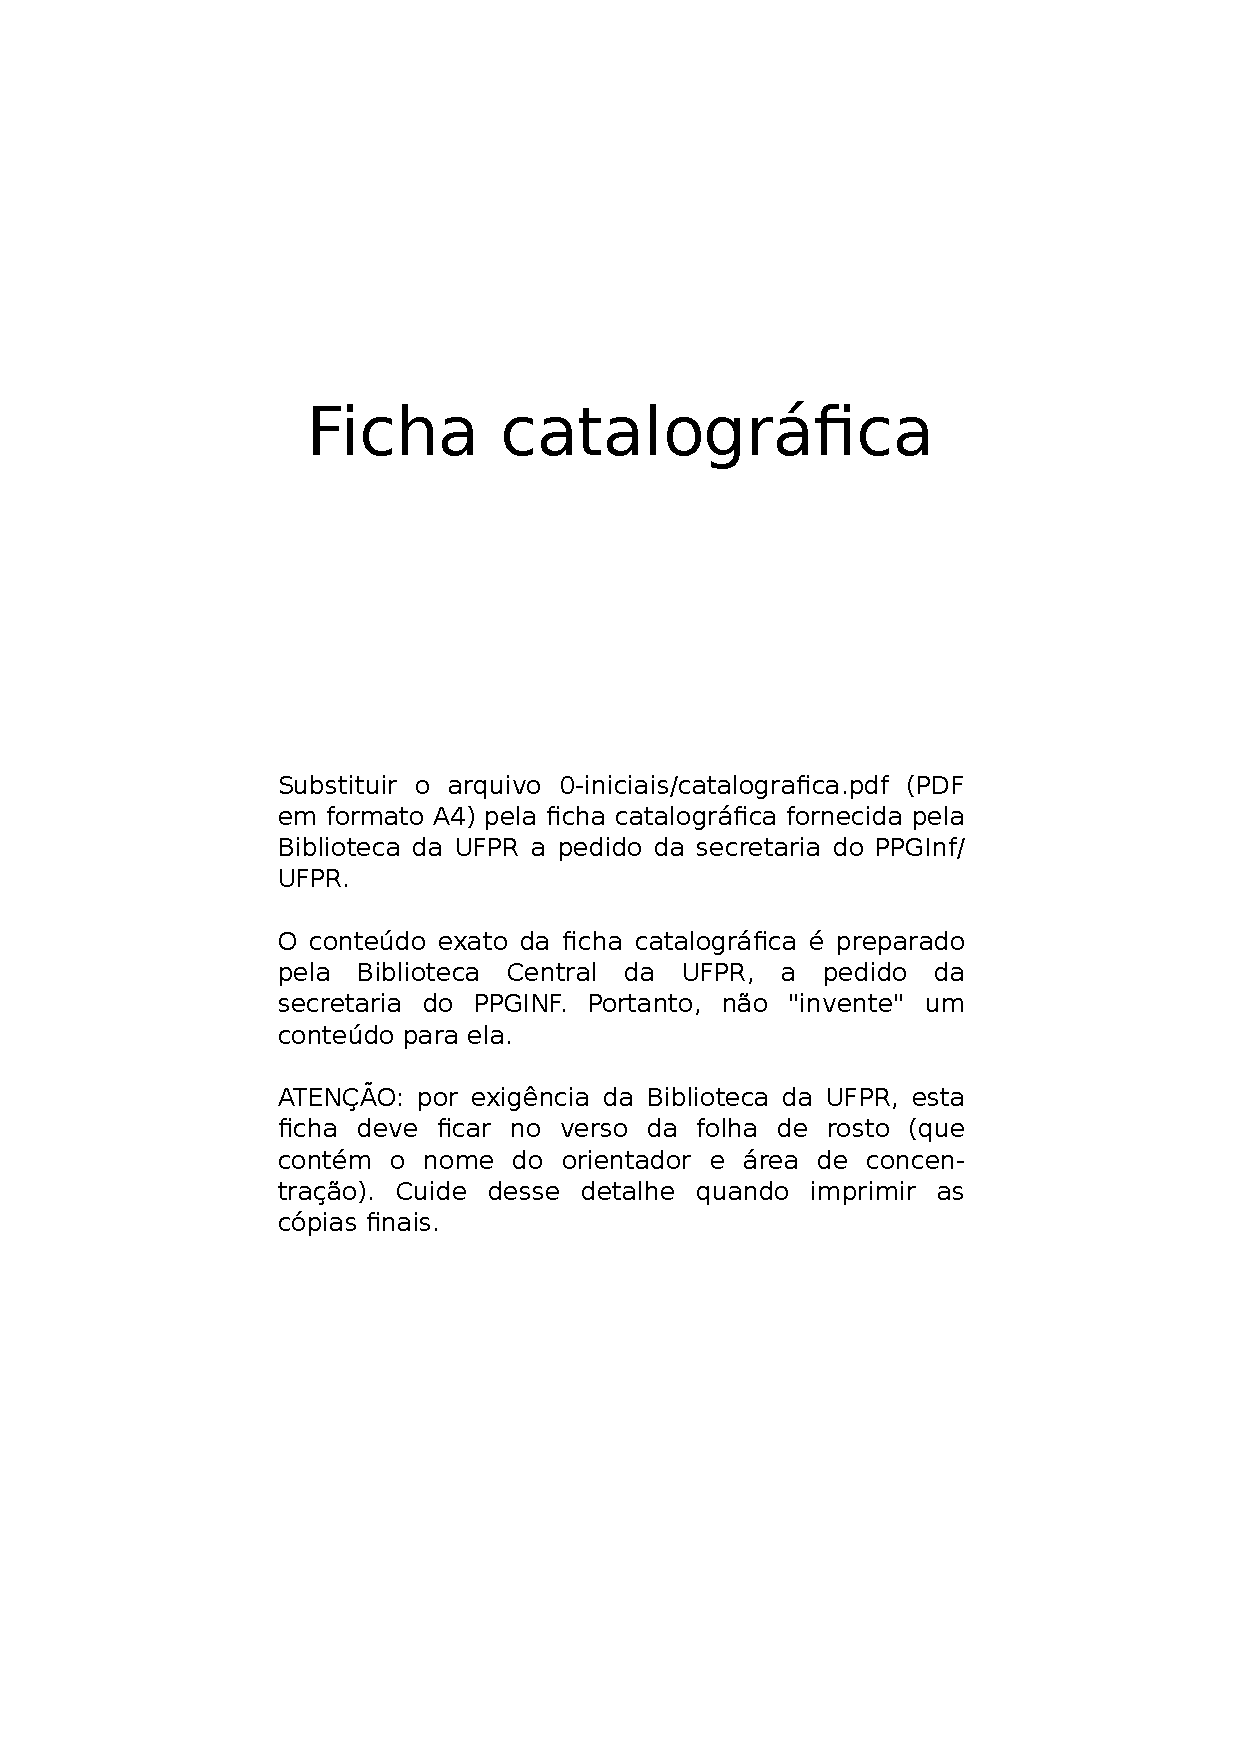
\includepdf[noautoscale]{0-iniciais/catalografica.pdf}

\end{ficha}

%=====================================================
	% ficha catalográfica
%% A ficha de aprovação será fornecida pela secretaria do programa,
% após a defesa e cumprimento dos demais trâmites legais.

\begin{aprovacao}	% só gera conteúdo se for na versão final

% inclusão do termo de aprovação final (arquivo PDF)
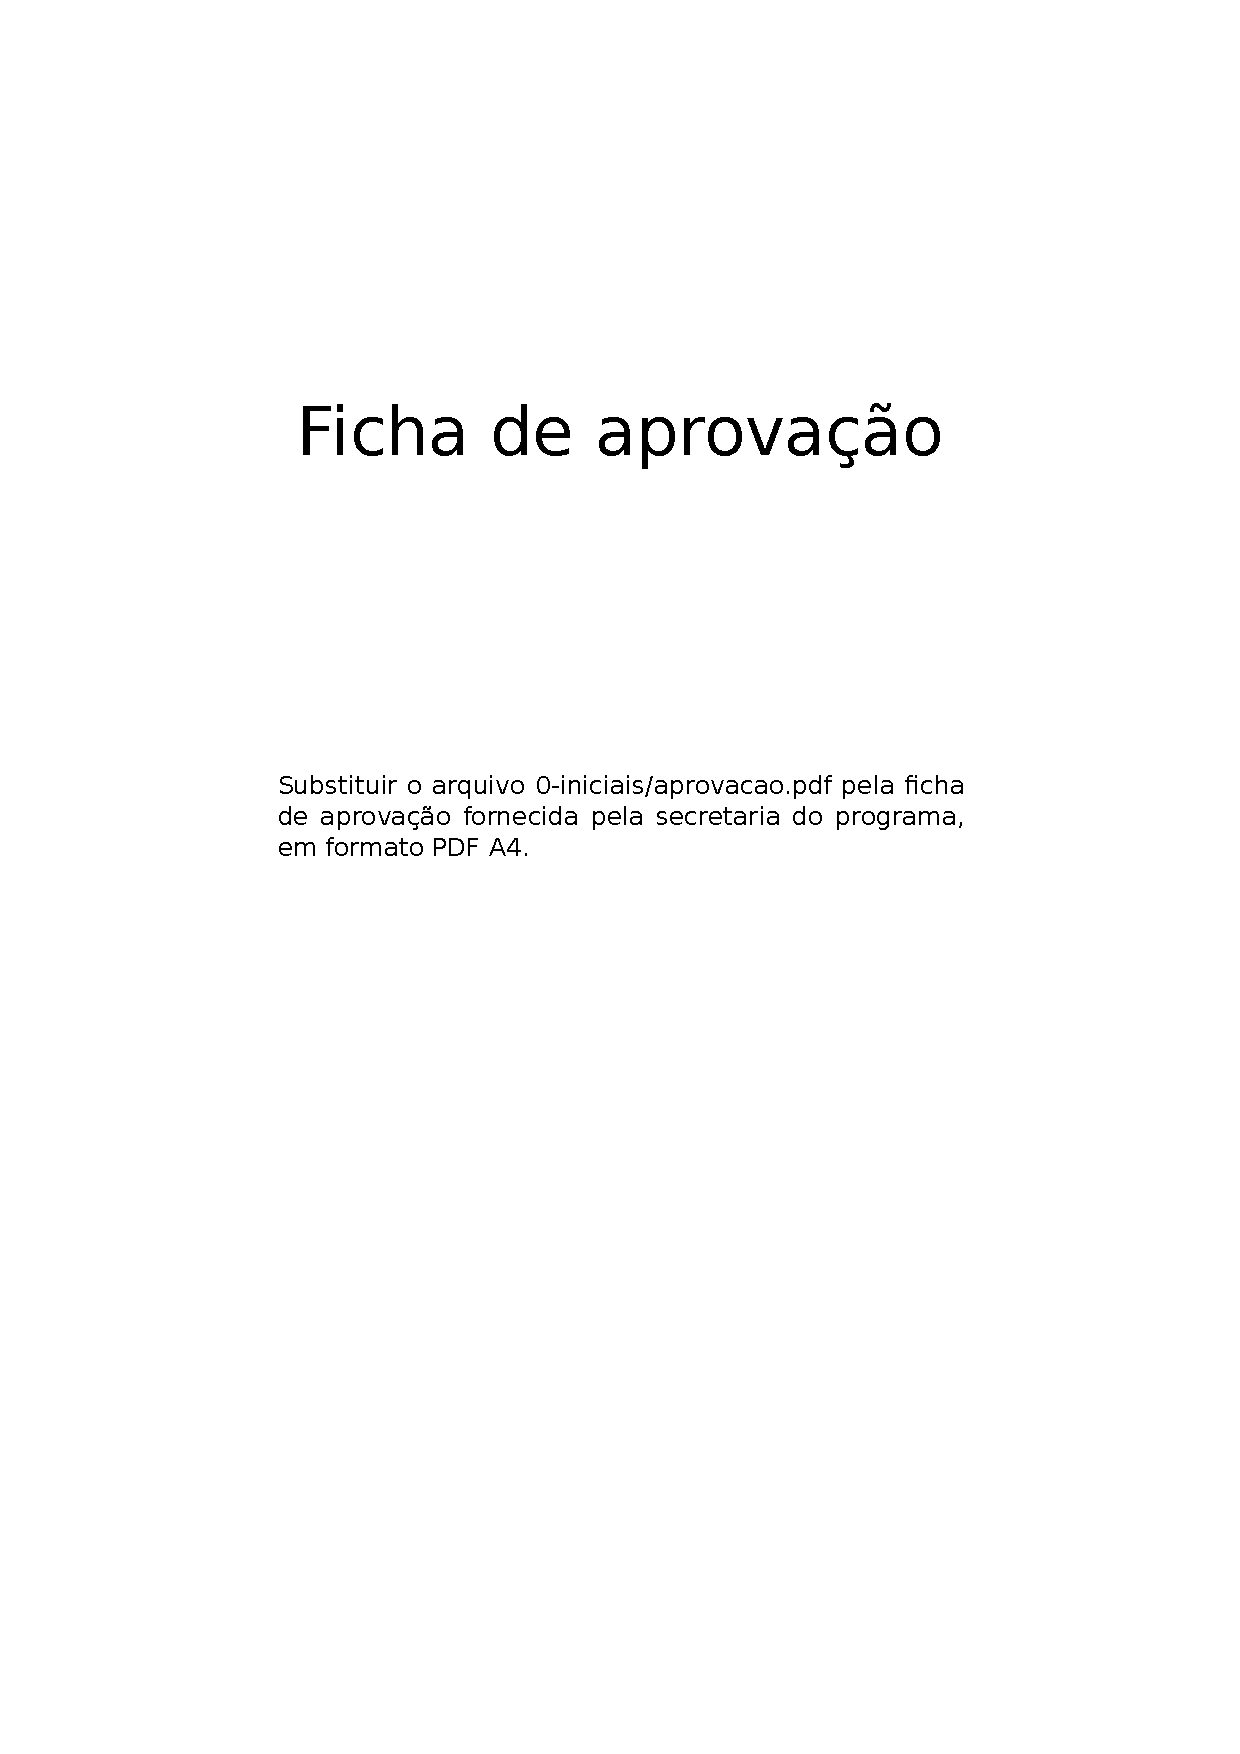
\includepdf[noautoscale]{0-iniciais/aprovacao.pdf}

\end{aprovacao}

%=====================================================
		% folha de aprovação
\begin{dedica}  % só gera conteúdo se for na versão final

A alguém...

\end{dedica}

		% dedicatória
\begin{agradece}	% só gera conteúdo se for na versão final

Inserir os agradecimentos. Os agradecimentos devem ocupar no máximo uma página, devem ser justificados na largura da página e com um afastamento de parágrafo na primeira linha de 1,27 cm. O espaçamento entre linhas deve ser de 1,5 linhas. Não deve haver espaçamento adicional entre parágrafos.

\lipsum[2-5]	% gera um texto aleatório

\end{agradece}

		% agradecimentos

% resumo (português) e abstract (inglês), nesta ordem
\begin{resumo}
Contexto

Problema

proposta de solução

Metodologia de avaliacao

%\lipsum[11-14]	% texto aleatório

\end{resumo}


\begin{otherlanguage}{english}

\begin{abstract}

% em inglês, o primeiro parágrafo não deve ser indentado
\noindent
Contexto

Problema


\end{abstract}

\end{otherlanguage}



% listas  de figuras, tabelas, abreviações/siglas, símbolos
\listoffigures
\clearpage
\listoftables
%=====================================================

% lista de acrônimos (siglas e abreviações)

\begin{listaacron}

\begin{longtable}[l]{p{0.2\linewidth}p{0.7\linewidth}}
DINF & Departamento de Informática\\
PPGINF & Programa de Pós-Graduação em Informática\\
UFPR & Universidade Federal do Paraná\\
CDN & \emph{Content Delivery Network}\\
\end{longtable}

\end{listaacron}

%=====================================================
		% ainda deve ser preenchida à mão
%=====================================================

% lista de símbolos

\begin{listasimb}

\begin{longtable}[l]{p{0.2\linewidth}p{0.7\linewidth}}
$\alpha$ & alfa, primeira letra do alfabeto grego\\
$\beta$ & beta, segunda letra do alfabeto grego\\
$\gamma$ & gama, terceira letra do alfabeto grego\\
$\omega$ & ômega, última letra do alfabeto grego\\
$\pi$ & pi \\
$\tau$ & Tempo de resposta do sistema\\
$\theta$ & Ângulo de incidência do raio luminoso\\
\end{longtable}

\end{listasimb}

%=====================================================
		% idem

% sumário
\tableofcontents

%=====================================================

% define estilo do corpo do documento (capítulos e apêndices)
\mainmatter
\pagestyle{mainmatter}

% inclusao de cada capítulo, alterar a gosto (do professor de Metodologia)
\chapter{Introdução}

%=====================================================

% A introdução geral do documento pode ser apresentada através das seguintes seções: Desafio, Motivação, Proposta, Contribuição e Organização do documento (especificando o que será tratado em cada um dos capítulos). O Capítulo 1 não contém subseções\footnote{Ver o Capítulo \ref{cap-exemplos} para comentários e exemplos de subseções.}.

\section{Contextualização}
Vivemos em um mundo rodeado de tecnologia, onde a cada dia somos surpreendidos com uma coisa totalmente inovadora, disruptiva. Uma era onde a internet foi respons\'avel por atravessar mares, superar dist\^ancias e at\'e mesmo idiomas. Hoje se pode comunicar em tempo real com pessoas que est\~ao em lados completamente oposto ao seu. 

Hoje \'e poss\'ivel que empresas estrangeiras muito distantes fisicamente, como China, India, EUA e etc, forne\c{c}am servi\c{c}os para regi\~oes mais remotas do mundo. Isso inclui servi{c}os de multim\'idia como armazenamento de fotos, de v\'ideos e at\'e conte\'udos de consumo instant\^aneo.

Esse encurtamento de dist\^ancia pode parecer simples, mas vem de um sistema complexo que visa fornecer ao usu\'ario final uma experi\^encia agrad\'avel com conte\'udos entregues de maneira satifat\'oria mas sem, necessariamente, replic\'a-lo por todo o globo. O que nos leva a dizer que uma CDN (\textit{Content Delivery Network}) \'e uma rede de distribui\c{c}\~ao de conte\'udo que tem como objetivo fornecer ao usu\'ario de aplica\c{c}\~oes globais uma experi\^encia satisfat\'oria na utiliza\c{c}\~ao de servi\c{c}os, principalmente sob demanda. Podemos ver alguns desses servi\c{c}os na figura \ref{figura:contextualizacao}.
\begin{figure}[H]
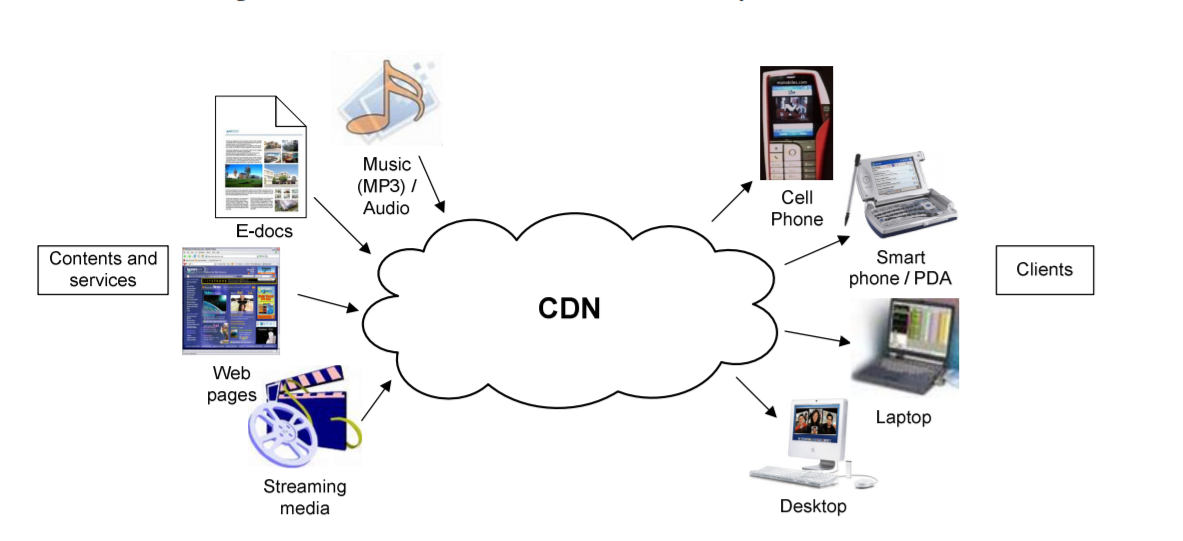
\includegraphics[height=7cm]{Figuras/contextualizacao.png}
\caption{Fornecedores x Consumidores} 
\label{figura:contextualizacao} 
\end{figure}
H\'a v\'arios servi\c{c}os que se utiliza no dia a dia onde essa no\c{c}\~ao de CDN \'e completamente abstrata ao usu\'ario final, como servi\c{c}os de Video-On-Demand de empresas de TV, spotify, Amazon Prime Video e at\'e Netflix, como \'e mostrado no artigo do \cite{adhikari2012unreeling}.

Existem hoje diversas empresas que fornecem esse servi\c{c}o ao redor do globo. Como Akamai, Limelight, Level 3 entre outras. Dessas redes a mais conhecida \'e a Akamai, que foi criada dentro do MIT (\textit{Massachusetts Institute of Technology}), e tem como clientes empresas como Adobe, \emph{Airbnb}, \emph{American Idol}, \emph{Audi} e muitas outras. Essas tr\^es redes s\~ao hoje as principais fornecedoras de servi\c{c}o de CDN. Cada uma com uma caracter\'istica e voltada para um p\'ublico.
\section{Problema}

Falar da questão de segurança e dificuldade de se garantir a segurança de um conteúdo que é distribuído em multiplas máquinas.
\section{Objetivos}

Resumidamente: Aprensentar uma solução que permite cifrar um conteúdo com a chave privada do fornecedor de conteúdo de forma que possa ser decifrado por qualquer usuário que tenha autorização.
\section{Estrutura do Documento}

Apresentar a estrutura do documento - Fazer por ultimo.
%=====================================================
			% introdução


\chapter{Redes de distribuição de conteúdo}
%\section{Composi\c{c}\~ao de uma \emph{Content Delivery Network}} 
\label{sec:composicao}

Para entendermos melhor uma Redes de distribuição de conteúdo (\emph{Content Delivery Network} - CDN), precisamos primeiro destrich\'a-la em v\'arios pequenos peda\c{c}os para assim compreendê-la em uma maneira global.

Uma CDN apesar de ,abstratamente, ser vista como um mecanismo \'unico, pode ser vista tamb\'em como a soma de v\'arios tipos de elementos e caracter\'isticas que somadas e configuradas formar\'a um mecanismo \'unico e transparente aos usu\'arios.

Fazem parte dessas caracter\'isticas: organiza\c{c}\~ao, tipos de servidores, protocolos e tipos de conte\'udo. Que serão detalhados nesse capítulo.

\section{Visão Geral}

\textcolor{red}{Generalizar CDNs em um paragrafo - Citar exemplos como Netflix, spotify e até serviços de noticias do android}

Quanto a organiza\c{c}\~ao uma CDN pode ser uma rede unicamente CDN ou uma rede \textit{overlay}, que nada mais \'e que uma rede onde ela tenta abstrai as camadas de redes j\'a existentes(como transporte, redes entre outras) e transforma-l\'a em uma rede puramente CDN.

Os tipos de conte\'udo que ir\~ao ser transportados dentro da rede s\~ao fundamentais para definir diversos aspectos de configura\c{c}\~oes que ser\~ao utilizadas dentro da rede. Como por exemplo, a forma de Cache que ser\~ao feitas os arquivos ou at\'e mesmo a forma como v\~ao ser distribu\'idos, se ser\~ao distribu\'idos em conjunto ou em partes. 

\section{Tipos de servidores}
\label{section:tipos_de_servidores}
Há dois tipos servidores: Servidor de origem e servidor de ponta. Isso independente de suas configurações físicas(quantidade de memória, CPU, HD e \emph{etc}).

\subsection{Servidores de origem}

S\~ao servidores de origem servidores onde toda a informa\c{c}\~ao que irá ser consumida fica baseado. \'E o lugar onde os conte\'udos v\~ao ser primeiramente armazenados e/ou gerados e é o ponto principal do sistema.

\'E ele o respons\'avel por, na aus\^encia da informa\c{c}\~ao perto do cliente, fornecer tudo o que o cliente necessita de informa\c{c}\~ao. Normalmente em primeiros acessos.

H\'a uma necessidade intr\'inseca de que esse servidor tenha excelentes configura\c{c}\~oes f\'isicas e \'otimas regras de seguran\c{c}as, \textit{firewall} a principal delas, que possam garantir a integridade do sistema mesmo em caso de muitos acessos.

\subsection{Servidores de ponta}
S\~ao servidores que mais pr\'oximos aos clientes. Parte do conte\'udo do servidor de origem estar\'a replicado nele. Dizemos em parte, pois n\~ao sabemos quais pol\'iticas de \textit{cache} que ser\'a adotada pelos criadores da rede. 
\\
Podemos ilustr\'a-los conforme a figura \ref{figura:tipos_servidores}.
\begin{figure}[H]
\caption{Tipos de servidores}
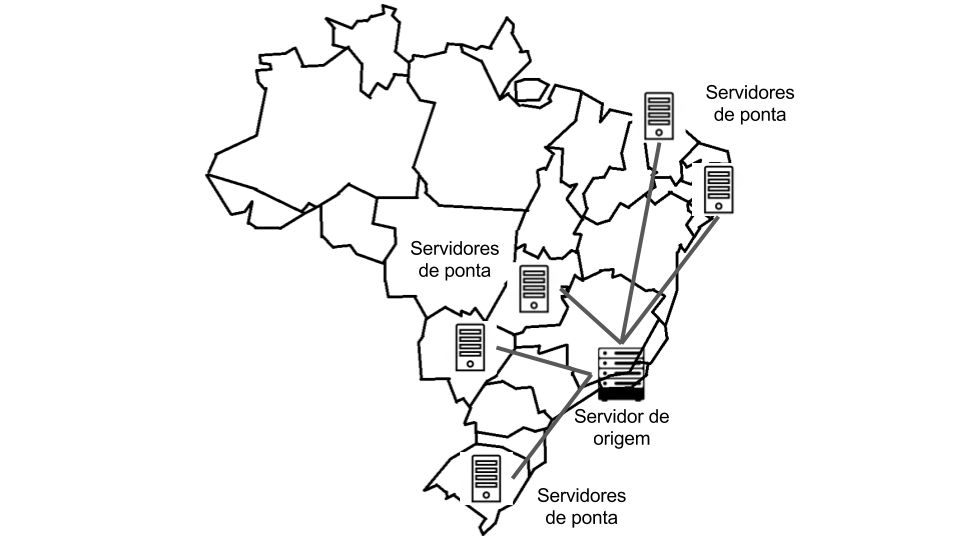
\includegraphics[height=9cm]{Figuras/tipos_servidores.png} 
\label{figura:tipos_servidores} 
\end{figure}

Vale salientar que esses \textit{status} de ser de ponta ou ser de origem não s\~ao imut\'aveis. Em ambientes reais e comerciais um servidor de origem \'e tamb\'em um servidor de ponta para um outro conte\'udo. Isso \'e o respons\'avel por tornar as grandes \emph{CDNs} completamente transparentes geograficamente perante aos seus clientes.
\section{Protocolos de intera\c{c}\~oes}
\label{section:protocolos_interacoes}
\begin{figure}[H]
\caption{Tipos de relacionamentos}
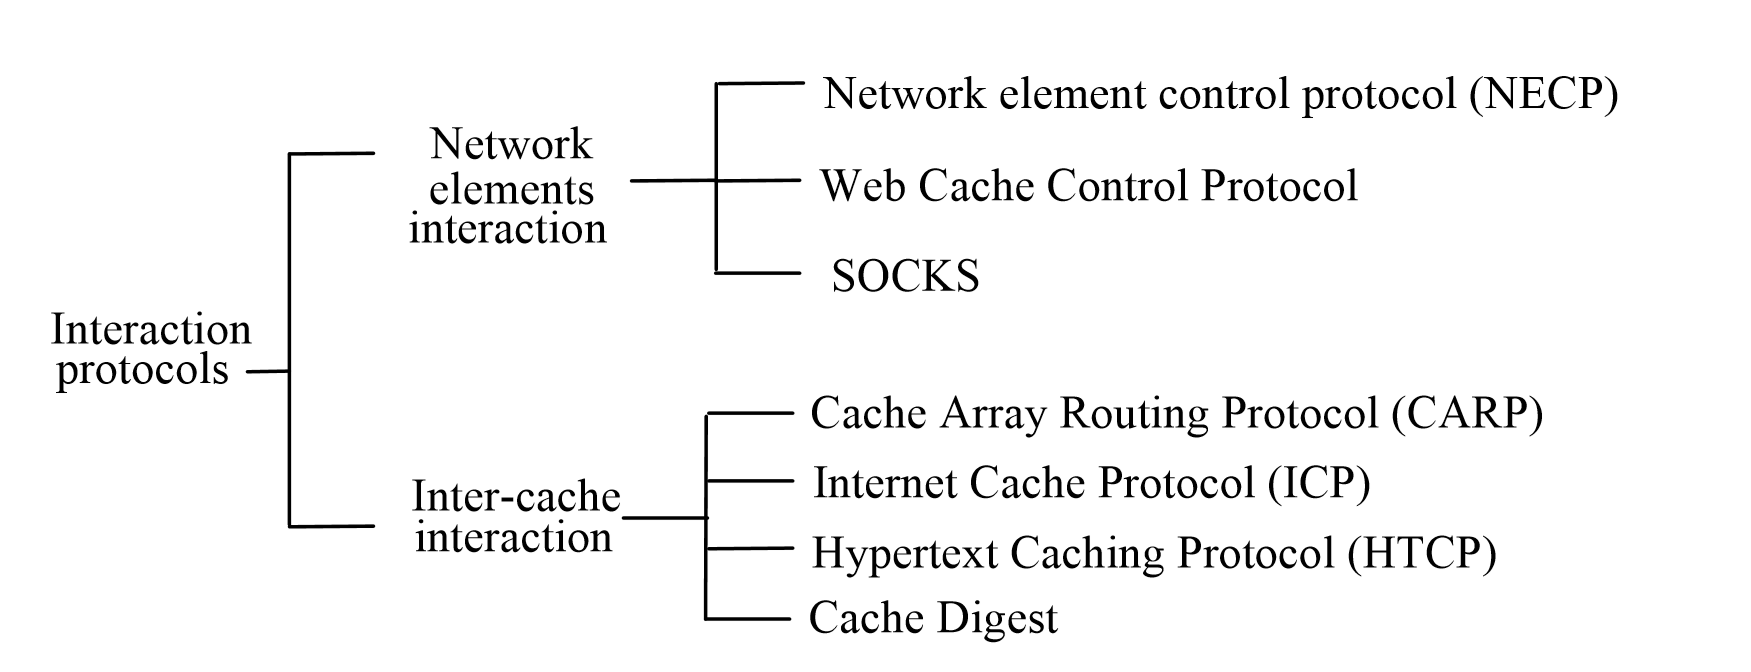
\includegraphics[width=15cm]{Figuras/tipos_relacionamentos.png} 
\label{figura:tipos_relacionamentos}
\end{figure}

Os protocolos de intera\c{c}\~oes podem ser divididos em duas partes: Protocolos de intera\c{c}\~oes de elementos da rede e Protocolos de intera\c{c}\~oes entre os servidores de cache da CDN. 


\subsection{Intera\c{c}\~oes dos elementos da rede}
\begin{figure}[H]
\caption{Tipos de protocolos de itera\c{c}\~oes}
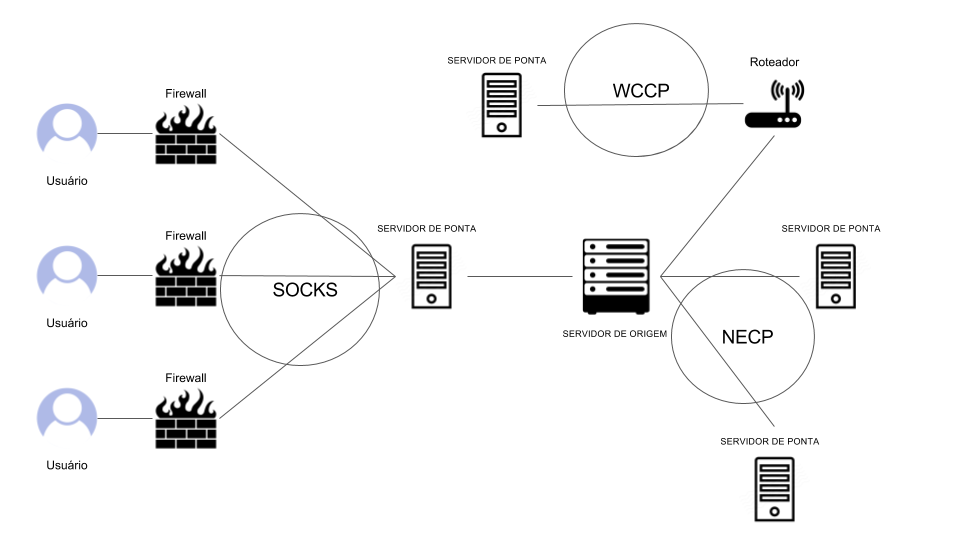
\includegraphics[height=9cm]{Figuras/protocolos_interacao_elementos.png} 
\label{figura:protocolos_interacao_elementos}
\end{figure}

Dentro dos protocolos de intera\c{c}\~oes dos elementos de rede podemos verificar que cada um possui sua especificidade e funcionalidade bem definida, como podemos ver na figura \ref{figura:protocolos_interacao_elementos} , tentando proteger n\~ao s\'o a rede mas tamb\'em o usu\'ario, o servidor, os roteadores e a comunica\c{c}\~ao entre os mesmos.
\paragraph{Socks} \'e um protocolo desenhado para um \textit{framework} para aplica\c{c}\~oes cliente-servidor que rodem em TCP ou UDP e utilizem os servi{c}os do \textit{firewall}. Sua principal funcionalidade \'e gerar um t\'unel de comunica\c{c}\~ao seguro entre cliente e servidor.
\paragraph{NECP} \'e um protocolo leve de comunica\c{c}\~ao que serve para sinalizar o tr\'afico entre os elementos da rede.
\paragraph{WCCP} serve para itera\c{c}\~oes entre roteadores e \textit{web-caches}	e tamb\'em para transporte entre os mesmos.


\subsection{Intera\c{c}\~oes de cache}

Os protocolos de intera\c{c}\~oes de cache s\~ao protocolos que organizam as trocas de informa\c{c}\~oes entre os servidores, ou seja, \'e ele que dita como ir\'a funcionar a distribui\c{c}\~ao da informa\c{c}\~ao dentro da rede.
 Conforme vimos na figura \ref{figura:tipos_relacionamentos}, e segundo \cite{pathan2007taxonomy}, existem 4 tipos de protocolos aplicados nessa circunst\^ancia como podemos ver na figura \ref{figura:protocolos_interacao_cache}
\begin{figure}[H]
\caption{Tipos de protocolos de itera\c{c}\~oes}
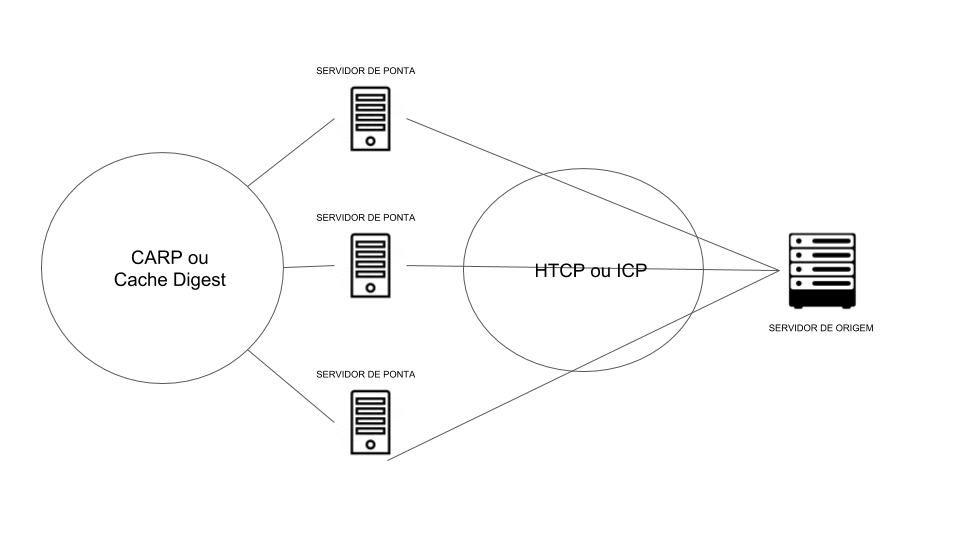
\includegraphics[height=9cm]{Figuras/protocolos_interacoes_cache.png} 
\label{figura:protocolos_interacao_cache}
\end{figure}

Dois deles s\~ao: HTCP - Hypertext Caching Protocol e ICP - Internet Cache Protocol que s\~ao concorrentes entre s\'i e tem como funcionalidade controlar o fluxo de informa\c{c}\~ao entre os caches. Sendo atrav\'es deles que se controla o que ir\'a para um determinado servidor de ponta, por exemplo. Falaremos mais sobre ambos em \ref{section:HTCP} e \ref{section:ICP} respectivamente.
 Existe tamb\'em os protocolos CARP -  Cache Array Routing Protocol e Cache Digest, tamb\'em concorrentes, servem para controlar o conte\'udo existente dentro de cada servidor e saber onde est\~ao os outros conte\'udos. Falaremos mais sobre ambos em \ref{section:CARP} e \ref{section:Cache Digest} respectivamente.

\subsection{HTCP}
\label{section:HTCP}
Como dito anteriormente o HTCP, Hypertext Caching Protocol, \'e um protocolo de intera\c{c}\~ao entre os caches, suas principais caracterist\'icas s\~ao:
\begin{itemize}
\item Protocolo para descobrir Caches HTTP;
\item Suporte ao HTTP 1.0;
\item Permite incluir cabeçalhos nas respostas;
\item Podem ser enviados via TCP/UDP;
\item Devem ser resilientes a falhas.
\end{itemize}

\subsection{ICP}
\label{section:ICP}
J\'a o ICP, Internet Cache Protocol, \'e um protocolo muito mais leve que possui as seguintes caracterist\'icas:
\begin{itemize}
\item Protocolo de mensagem leve;
\item Utilizado para comunica\c{c}\~ao de Caches;
\item Utiliza consultas para determinar localiza\c{c}\~ao mais apropriada;
\item Suporte ao HTTP 0.9;
\item Comunica-se com caches vizinhos;
\item recebe MISS ou HIT como resposta;
\item Enviado via UDP;
\item Falha por timeout indica caminho quebrado;
\item Fornece informa\c{c}\~oes para balanceamento atrav\'es das medidas de perda.
\end{itemize}

\subsection{HTCP x ICP}
Analisando os dois protocolos HTCP e ICP, podemos fazer um quadro comparativo entre eles e coloc\'a-los da seguinte maneira(figura \ref{figura:htcp_x_icp}):

\begin{figure}[H]
\caption{HTCP x ICP}
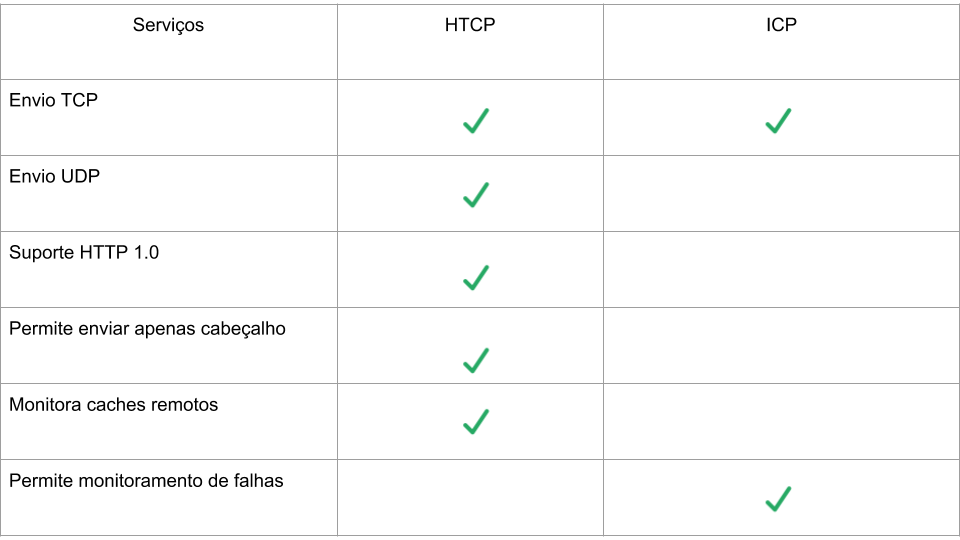
\includegraphics[height=9cm]{Figuras/htcp_x_icp.png} 
\label{figura:htcp_x_icp}
\end{figure}

\subsection{CARP}
\label{section:CARP}
CARP -  Cache Array Routing Protocol
 Protocolo de armazenamento distribu\'ido baseado em uma lista conhecida de proxies fracamente acoplada e uma fun\c{c}\~ao hash para dividir o espa\c{c}o URL entre esses proxies.
\begin{itemize}
\item Cliente HTTP pode enviar requisi\c{c}\~ao \`a qualquer proxy da lista.
\end{itemize}

\subsection{Cache Digest}
\label{section:Cache Digest}
Protocolo de interc\^ambio e formato de dados entre caches.
\begin{itemize}
\item Fornece um resumo dos conte\'udos na resposta;
\item Soluciona os problemas de congestionamento e timeout;
\item Torna poss\'ivel determinar se um servidor possui em cache um conte\'udo;
\item Executado via HTTP ou FTP;
\item Cont\'em tempo de expira\c{c}\~ao na resposta;
\item Pode ser utilizados para eliminar redund\^ancia.
\end{itemize}

\section{Sele\c{c}\~ao e entrega de conte\'udo}
\label{section:selecaoentrega}
Dentro de uma CDN temos que  nos preocupar com a forma como esse conte\'udo vai catalogado, armazenado e distribu\'ido dentro da rede, o que vimos no item \ref{section:protocolos_interacoes}, como tamb\'em temos que nos preocupar como esse conte\'udo vai chegar at\'e o cliente (usu\'ario) da forma mais otimizada poss\'ivel, ou seja, o servidor o qual vai fornecer as informa\c{c}\~oes para ele ser\'a o mais perto ou mais r\'apido. 
 Temos que destacar tamb\'em a import\^ancia da otimiza\c{c}\~ao do fluxo de informa\c{c}\~ao pela rede. Visto que quanto maior o tr\'afico de informa\c{c}\~ao pela rede significa que a informa\c{c}\~ao est\'a mais distante do usu\'ario e tamb\'em que vai ter um custo maior pela troca intensa de informa\c{c}\~ao. 
 Segundo \cite{krishnamurthy2001use}, na tentativa de otimizar o redirecionamentos de URL para o usu\'ario se sacramentou dois tipos de t\'ecnicas de redirecionamentos, Full - site e Partial - site.

\subsection{Full - site}
Na t\'ecnica de Full-site todo o conte\'udo \'e entregado ao usu\'ario de um servidor ponta \'unico. Ou seja, o usu\'ario faz uma requisi\c{c}\~ao ao servidor principal, onde o mesmo processa um algoritmo de roteamento para encontrar o servidor ponta que melhor se enquadra como resposta, e ent\~ao retorna ao usu\'ario o endere\c{c}o onde ent\~ao ser\'a consumido por fim todas as informa\c{c}\~oes requisitadas. 
 \'E importante salientar que essa t\'ecnica \'e amplamente utilizada por servi\c{c}os que fazem pouco uso de dados da rede. Uma p\'agina est\'atica da web, por exemplo, se encaixaria perfeitamente nesse contexto. Visto que possui baixo grau de modifica\c{c}\~oes e seu tamanho \'e pequeno perto de outros tipos de m\'idias que circulam na web.

\subsection{Partial - site}
J\'a redirecionamentos do tipo Partial-sites os servidores principais retornam para o usu\'ario uma parte do conte\'udo e disparam, automaticamente, um algoritmo de roteamento para encontrar o restante da informa\c{c}\~ao e retornar ao usu\'ario. Conforme podemos ver na figura \ref{figura:entrega_conteudo}
\begin{figure}[H]
\caption{Entrega de conte\'udo}
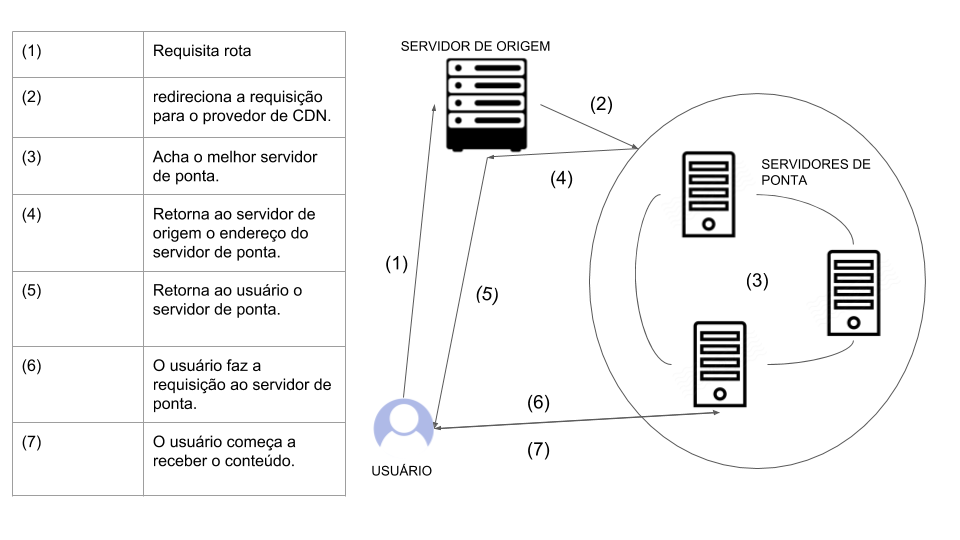
\includegraphics[height=9cm]{Figuras/entrega_conteudo.png} 
\label{figura:entrega_conteudo}
\end{figure}
Nela podemos ver que todo o processo acontece em basicamente sete etapas. (1) o usu\'ario faz uma requisi\c{c}\~ao ao servidor principal onde este dispara (2) um roteamento (3) para buscar qual \'e o melhor servidor para aquele usu\'ario. Depois, em (4) o servidor principal recebe a identifica\c{c}\~ao do servidor de ponta e repassa ao usu\'ario (5) juntamente com um arquivo que cont\'em as informa\c{c}\~oes centrais que normalmente s\~ao iguais para o mundo todo. Em seguida o usu\'ario come\c{c}a a enviar (6) e receber (7) informa\c{c}\~oes com o servidor de ponta.

 Entretanto h\'a em (3) diversas formas de fazer esse roteamento quanto a distribui\c{c}\~ao do conte\'udo pela rede e quanto a aglomera\c{c}\~ao desse conte\'udo dentro do servidores de cache. 
 Tipo de distribui\c{c}\~ao nada mais \'e do que a forma como o conte\'udo vai ser disperso na rede, como esse conte\'udo vai se aproximar do n\'o que est\'a mais perto do usu\'ario. 

Os tipos de distribui\c{c}\~ao mais frequentemente utilizados s\~ao o emp\'irico e o por popularidade.

Emp\'irico trata, como o pr\'oprio nome diz, de uma forma de distribui\c{c}\~ao sem nenhum conhecimento espec\'ifico a respeito, utilizando-se apenas um conhecimento experimental de onde seria melhor posicionado o conte\'udo.
 Em um esquema baseado em popularidade a distribui\c{c}\~ao \'e feita conforme a notoriedade. Ou seja, quanto maior o n\'umero de requisi\c{c}\~oes a um conte\'udo, mais ele ser\'a distribu\'ido nos servidores de ponta perto do usu\'ario.
 Ambos esquemas n\~ao s\~ao necessariamente excludentes, pode-se inicialmente aplicar a forma empir\'ica para gerar dados a respeito da distribui\c{c}\~ao e depois utilizar esses dados para aplicar o modo de popularidade.
	
Tamb\'em existe as formas de aglomera\c{c}\~oes de conte\'udo. Isso existe porque os conte\'udos podem ser conjuntos de objetos ou objetos independentes. 
As formas de aglomera\c{c}\~oes s\~ao por objeto e por conjunto de objetos.

Aglomera\c{c}\~ao por objeto vai juntar os objetos mais selecionados e distribu\'i-los individualmente entre os servidores. J\'a por conjunto de objetos ele vai separ\'a-los em grupos e distribui-los em conjuntos. 
 Podemos exemplicar da seguinte forma: Em um site temos v\'arios elementos, temos o HTML, temos o CSS e temos a m\'idia de um v\'ideo qualquer. Podemos separar da seguinte forma: temos 3 elementos onde 2 deles s\~ao altamente dependentes(HTML e CSS) e temos 1 que pode ser diferente em cada regi\~ao do pa\'is, que \'e o v\'ideo. 
 Ent\~ao podemos misturar as formas de aglomera\c{c}\~oes. Para o HTML e para o CSS agrupamos em conjuntos de objetos; e para o v\'ideo fazemos a aglomera\c{c}\~ao por objeto,j\'a que ser\'a distribu\'ido de maneira independente nos servidores.

Analisando os tipos,perceber-se que nenhuma das op\c{c}\~oes s\~ao excludentes entre s\'i, pode-se combinar quaisquer tipo de distribui\c{c}\~ao e aglomera\c{c}\~ao e as escolhas v\~ao depender das necessidades de cada aplica\c{c}\~ao.\'E necess\'ario uma an\'alise minuciosa de cada aplica\c{c}\~ao para chegar em um veredito da melhor abordagem.
\subsection{VOD}
\label{subsec:vod}
\paragraph{VOD - Video on Demand} - Segundo \cite{garfinkle1996video}, \'e um sistema de que proporciona uma interface de comunica\c{c}\~ao com o usu\'ario de produtos dispon\'iveis de uma esta\c{c}\~ao central remota.
 \'E um sistema muito utilizado por operadoras de conte\'udo onde \'e o cliente quem decide o hor\'ario que ir\'a consumir determinado conte\'udo.
 Isso permite \`as pessoas que tinham que esperar o hor\'ario certo para consumir determinado conte\'udo, poderem a qualquer momento e em qualquer lugar fazer uso do mesmo.
\paragraph{Microsoft Smooth Streaming} \'E um sistema de consumo de v\'ideo onde a qualidade do v\'ideo transmitida vai ser definida conforme a qualidade da banda dispon\'ivel. Clientes que possuem alta disponibilidade de banda ter\~ao maior qualidade do v\'ideo. 
 Para conseguir tocar um v\'ideo nesse formato o player do usu\'ario tem que ser capaz de interpretar um manifesto que cont\'em dentro de outras coisas, o caminho de onde est\'a localizado a m\'idia desejada. 
 J\'a para conseguir fazer a transi\c{c}\~ao de qualidade o v\'ideo \'e quebrado em pequenos peda\c{c}os chamados de "chunks". Ent\~ao, conforme \'e verificada um aumento ou decremento da banda dispon\'ivel o player come\c{c}ar que consumir chunks de qualidade diferente da atual alternando assim o \textit{bitrate} do v\'ideo que est\'a sendo consumido. 
 No artigo \cite{zambelli2009iis} podemos ver todas as aplica\c{c}\~oes e implica\c{c}\~oes dessa forma de consumo de m\'idia.
\subsection{VOD na pr\'atica}
\label{subsubsection:vod_exemplo}
Agora vamos ilustrar com um exemplo mais pr\'atico. Utilizaremos uma requisi\c{c}\~ao de uma URL de um VOD (Video On Demand) onde a parte de roteamento \'e feita no usu\'ario. A aplica\c{c}\~ao do usu\'ario faz uma requisi\c{c}\~ao \`a CDN e enquanto o cabe\c{c}alho da resposta n\~ao for 200 ele vai ler um campo dentro do cabe\c{c}alho de resposta e fazer uma nova requisi\c{c}\~ao. A figura  \ref{figura:vod_redirect_exemple} ilustra a situa\c{c}\~ao.

\begin{figure}[H]
\caption{Redirecionamento de CDN}
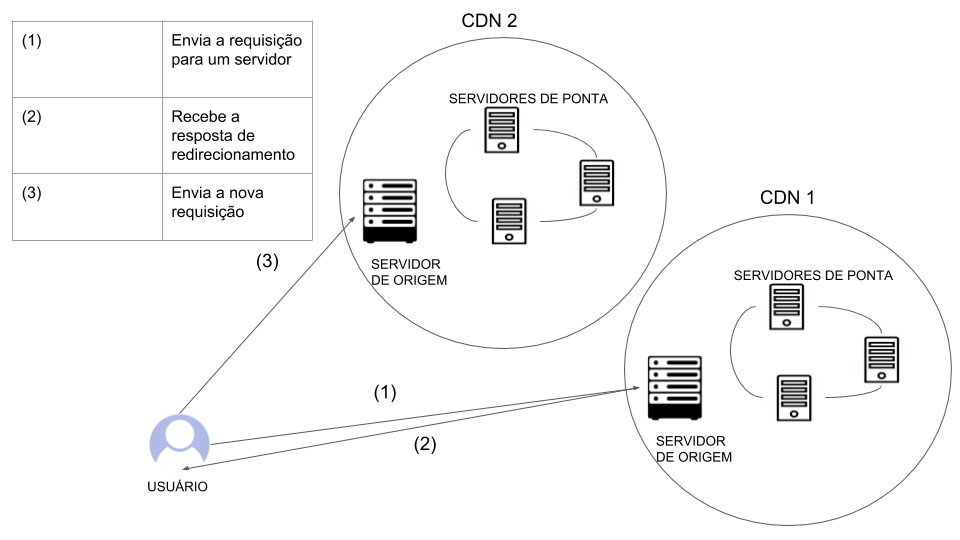
\includegraphics[width=15cm]{Figuras/vod_redirect_exemple.png} 
\label{figura:vod_redirect_exemple}
\end{figure}

\section{Considerações Finais}

Redes CDNs apesar de serem quase transparentes aos usuários não signfica que são simples. Como vimos possuem diversas características que devem ser levadas em consideração ao serem montadas ou estudadas. Em cada característica dessa é possível desenvolver diversos tipos de pesquisas.

Nesse trabalho iremos focar somente na entrega do conteúdo desejado (\ref{section:selecaoentrega}). Especificamente quanto a entrega de conteúdo de VOD (\ref{subsubsection:vod_exemplo}).
\chapter{Desafios de segurança de CDN}
\label{sec:seguranca}
 Podemos definir seguran\c{c}a como um conjunto de a\c{c}\~oes que e dos recursos utilizados para proteger algo ou algu\'em, ou, o que serve para diminuir os riscos ou perigo. Portanto, seguran\c{c}a \'e um tema extramente abrangente e complexo. Podemos falar de t\'opicos como seguran\c{c}a f\'isica, social, de um sistema ou at\'e mesmo de um grupo de servidores interconectados, que \'e o caso da CDN, e ainda coloca-los todos dentro do mesmo grupo. Ou seja, podemos trat\'a-los de forma separada ou analisando o conjunto todo.
 
Ainda dentro de Seguran\c{c}a de CDN podemos tratar de pontos principais, onde o vazamento \'e ponto crucial e mais l\'ogico de ser atacado. 
\begin{figure}[H]
\caption{Objetivos da seguran\c{c}a}
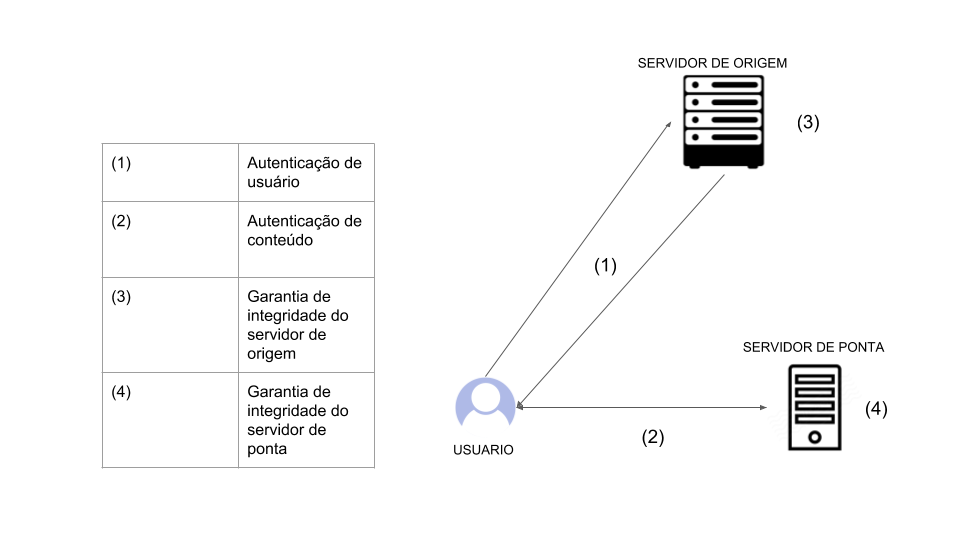
\includegraphics[height=9cm]{Figuras/seguranca_intro.png} 
\label{figura:seguranca_intro}
\end{figure}

Como vemos na figura \ref{figura:seguranca_intro} podemos observar que se tem quatro grandes pontos a serem garantidos em uma rede. Dois deles (1) e (2) de autentica\c{c}\~ao e outros dois (3) e (4) relacionados a integridade. O primeiro trata-se da autentica\c{c}\~ao de usu\'ario que \'e capacidade do sistema de garantir que aquele usu\'ario que est\'a acessando o conte\'udo tem mesmo os requisitos para acess\'a-lo. Ou seja, \'e mesmo um usu\'ario do sistema. Por ser um tema bem abrangente ser\'a tratado com mais profundidade em \ref{subsection:autenticacao_usuario}.

Em segundo lugar temos a autentica\c{c}\~ao de conte\'udo. Que \'e a garantia que o conte\'udo acessado \'e o mesmo buscado pelo usu\'ario, que o usu\'ario tem acesso a ele e tamb\'em \'e um conte\'udo que faz parte da rede de disponibilidade da CDN(que n\~ao \'e um conte\'udo inserido por terceiro sem autoriza\c{c}\~ao pr\'evia). Tudo isso tem que ser minuciosamente tratado e averiguado antes de retornar ao usu\'ario. Tudo isso ser\'a abordado em \ref{subsection:autenticacao_conteudo}.

Nos dois outros, (3) e (4), trata-se da seguran\c{c}a dos servidores. A\'i podemos falar de seguran\c{c}a f\'isica e l\'ogica. Tem-se que levar em conta a forma de acesso de cada um na hora de mensurar os aspectos de seguran\c{c}a de cada um deles. 

No servidor de origem se tem um acesso via HTTP, com um endereço "leg\'ivel". Esse acesso se dar\'a muitas vezes por v\'arias parte do globo, tendo que deix\'a-lo dispon\'ivel , portanto, vulner\'avel \`a diversos tipos de ataque, o que o torna extremamente complexo na hora de definir suas regras de seguran\c{c}a, n\~ao basta apenas subir um \textit{firewall} bloqueando m\'ultiplos acessos, \'e preciso saber exatamente os tipos de aplica\c{c}\~oes que ser\~ao tratadas para assim come\c{c}ar a desenhar as regras de \textit{firewall} que ser\~ao aplicadas.

J\'a no servidor de ponta a preocupa\c{c}\~ao com o acesso via HTTP j\'a \'e uma coisa a menos, visto que muitas vezes o acesso funcionar\'a via redirecionamento do servidor de origem, sendo o controle de endere\c{c}o feito pelo o mesmo. Mas h\'a diversos outros aspectos que tem que serem levados em conta, como parte da autentica\c{c}\~ao de conte\'udo para o usu\'ario, que nada mais \'e que garantir que o usu\'ario para o qual est\'a sendo enviado o conte\'udo tem acesso ao mesmo. Outra grande preocupa\c{c}\~ao \'e quanto a sua disponibilidade, pois \'e necess\'ario que o mesmo esteja "de p\'e" quando for requisitado conte\'udo e que durante o processo de transfer\^encia, caso haja alguma interrup\c{c}\~ao a mesma seja informada ao servidor de origem e o usu\'ario transferido para outro servidor sem que haja muitos danos \`a experi\^encia. Isso sem contar nas enumeras preocupa\c{c}\~oes que se deve ter com servidores. No livro \cite{stallings1995network} se pode aprofundar um pouco mais nessas quest\~oes de segurança na \textit{web}.

Mas para se aprofundar um pouco mais dentro dos conceitos de seguran\c{c}a de usu\'ario e conte\'udo de uma CDN \'e necess\'ario primeiro conhecer um pouco sobre protocolos AAA que ser\'a tratado em \ref{subsection:AAA}.
\section{protocolos AAA - Authentication, Authorization, and Accounting}
\label{subsection:AAA}
A associa\c{c}\~ao dos protocolos de autentica\c{c}\~ao, autoriza\c{c}\~ao e auditoria em um termo, protocolos AAA, se deu porque na maioria dos sistemas seguros esses tr\^es protocolos s\~ao extremamente necess\'arios e amplamente utilizados. em \cite{metz1999aaa} se pode aprofundar melhor. Mas vamos h\'a uma r\'apida s\'intese dos mesmos.
\paragraph{Autentica\c{c}\~ao}- Verifica a identidade digital do usu\'ario de um sistema, que segundo \cite{metz1999aaa}, envolve a valida\c{c}\~ao da identidade do usu\'ario final afim de permitir seu acesso \`a rede.

Esse procedimento \'e baseado na apresenta\c{c}\~ao de uma identidade junto com uma ou mais credenciais, que podem ser senhas, certificados digitais e etc.
\paragraph{Autoriza\c{c}\~ao}- \'E a concess\~ao de uso para determinados servi\c{c}os. Essa etapa s\'o \'e acionada mediante a autentica\c{c}\~ao pr\'evia de um usu\'ario. Ela leva em conta a identidade, o servi\c{c}o requerido e o estado atual do sistema. Muitas vezes ela trabalha com a utiliza\c{c}\~ao de filtros para retornar que tipo de protocolos ou aplica\c{c}\~oes s\~ao suportadas.

Na maioria dos casos os protocolos de autentica\c{c}\~ao e autoriza\c{c}\~ao trabalham juntos. Onde um depende diretamente do funcionamento do primeiro. Em ambientes de VOD, como se foi apresentado em \ref{subsubsection:vod_exemplo}, essa etapa normalmente \'e verificada nos servidores de ponta, os quais s\~ao respons\'aveis por fornecer o conte\'udo ao usu\'ario.
\paragraph{Auditoria}- A \'utima etapa do processo \'e relacionada a coleta de informa\c{c}\~oes de tr\'afego utilizado pelo usu\'ario. 

H\'a dois tipos de coletas: coletas em tempo real e coleta \textit{batch}. A primeira se refere a informa\c{c}\~oes captadas em tempo de uso, ou seja, enquanto o usu\'ario faz uso da rede essas informa\c{c}\~oes s\~ao enviadas. J\'a a segunda se refere a uma coleta que \'e primeiro armazenada e enviadas posteriormente. 

S\~ao essas informa\c{c}\~oes que s\~ao utilizadas pelas operadoras para cobran\c{c}a e taxa\c{c}\~ao do servi\c{c}os de VOD.
\section{Autentica\c{c}\~ao de usu\'ario}
\label{subsection:autenticacao_usuario}
A autentica\c{c}\~ao de usu\'ario envolve a a certeza que o usu\'ario que est\'a consumindo o conte\'udo ou tentando acessar a rede \'e o mesmo usu\'ario que tem acesso \`a aplica\c{c}\~ao. E o que acontece quando o usu\'ario faz login somente uma vez (em uma p\'agina)? Como garantir que \'e o mesmo usu\'ario?

Bom, a forma de armazenamento vai depender muito de onde est\'a sendo acessada a aplica\c{c}\~ao. Se for de um desktop, dentro de um navegador, normalmente vai ser armazenada dentro do \textit{cookies} do navegador. Se for de uma aplica\c{c}\~ao mobile, ou at\'e mesmo de uma aplica\c{c}\~ao desktop (sem ser um navegador), normalmente fica em alguma pasta tempor\'aria que \'e guardada pela mem\'oria \textit{flash}. Ent\~ao significa que uma vez feito login ele fica pra sempre armazenado?

N\~ao. Essas autentica\c{c}\~ao s\~ao tempor\'arias, muitas vezes com tempo de expira\c{c}\~ao definido pelas pr\'oprias aplica\c{c}\~oes, e requerem renova\c{c}\~ao da licen\c{c}a ou reautentica\c{c}\~ao do usu\'ario. 

Em todos os casos, h\'a diversas formas de autentica\c{c}\~ao dentro de sistemas computacionais. H\'a autentica\c{c}\~ao por login (normalmente email) e senha, por biometria, \textit{token} entre outras. Mas em aplica\c{c}\~oes \textit{web} login/senha s\~ao as mais utilizadas.

As etapas de verifica\c{c}\~ao de quantidade de aparelhos e a origem dos IPs de requisi\c{c}\~ao normalmente s\~ao feitas aqui.

Nesse processo \'e importante salientar tamb\'em a autentica\c{c}\~ao dos \textit{devices}. Nesse processo \'e muito importante que os \textit{devices} sejam limitados para que n\~ao haja vazamento de usu\'arios utilizando m\'ultiplas sess\~oes em mais de um dispositivo, quebrando assim a regra de que os acessos dos usu\'arios n\~ao podem serem compartilhados.

Na figura \ref{figura:autenticacao_conteudo} podemos v\^e quais processos, dentro do \textit{browser} , se comunicam com quais servidores.
\begin{figure}[H]
\caption{Comunica\c{c}\~ao: Processos x Servidores}
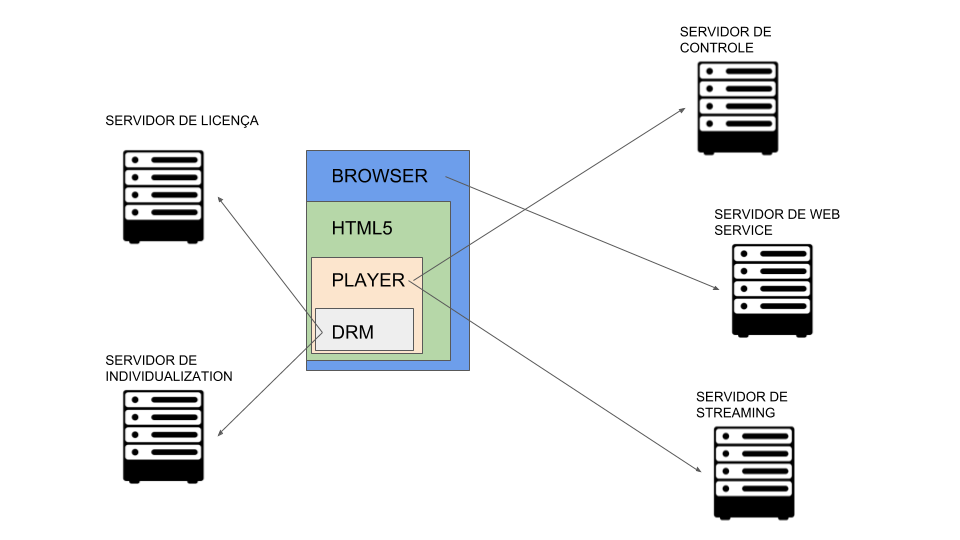
\includegraphics[width=14cm]{Figuras/autenticacao_conteudo.png} 
\label{figura:autenticacao_conteudo}
\end{figure}
\section{Certifica\c{c}\~ao de licen\c{c}as de conte\'udo}
\label{subsection:autenticacao_conteudo}
Dentro de certifica\c{c}\~ao de licen\c{c}as de conte\'udo h\'a uma gama de valida\c{c}\~oes que s\~ao ou que podem ser utilizadas, \cite{wein2012content} e \cite{leighton2007html} s\~ao duas delas.

Aqui iremos focar em uma chamada \textit{control DRM-encoded}, que \'e o m\'etodo mais utilizado hoje em dia. Utilizado inclusive por sistemas como Netfilx e VOD de operadoras de TV.

Esse processo est\'a intrinsecamente ligado ao processo de autentica\c{c}\~ao de usu\'ario explicado anteriormente. Nele o conte\'udo passa por uma s\'erie de valida\c{c}\~oes antes de tocar.

A primeira etapa do processo para tocar o conte\'udo \'e a etapa de \textbf{\textit{License Acquisition}}. Nela, apresentado por \cite{pomelo2009analysis}, antes de tocar \'e feito:
\begin{itemize}
\item Passo 1 -  A aplica\c{c}\~ao requisita do servidor um peda\c{c}o do conte\'udo. Este o retorna com o conte\'udo criptografado.
\item Passo 2 - O cliente l\^e o cabe\c{c}alho do conte\'udo criptografado e determina que aquele conte\'udo \'e criptografado. Para descriptografar o conte\'udo \'e necess\'ario que este tenha recebido a chave do servidor de licen\c{c}a. Caso n\~ao tenha recebido ele envia uma requisi\c{c}\~ao para adquiri-la. Se for a primeira vez que \'e feita a valida\c{c}\~ao da chave ele passa por um processo de \textit{individualization}. Que ser\'a explicado logo mais a frente.(figura \ref{figura:individualization}).
\item Passo 3 - O cliente recebe a licen\c{c}a do servidor, que antes de enviar a chave faz todo o processo de autencidade necess\'ario.
\item Passo 4 - O cliente ap\'os receber a chave pode tocar o conte\'udo. Isso se ele estiver licen\c{c}a para tal, \'e claro.
\end{itemize}

No passo 1 fica claro entender quando em \ref{subsec:vod} explicamos como \'e composto um VOD e qual o seu fluxo de comportamento.

O disparo do fluxo do \textit{individualization} \'e feito pela pr\'opia aplica\c{c}\~ao do cliente, que verifica caso o cliente n\~ao possua nenhuma licen\c{c}a ele aponta para um terceiro servidor, onde esse vai retornar com uma licen\c{c}a individual que ser\'a utilizada na hora de validar e tocar conte\'udo. O fluxo do processo \'e apresentado na figura \ref{figura:individualization}. 

Todo esse processo de troca de informa\c{c}\~oes \'e feito utilizando trocas de chaves assim\'etricas p\'ublicas garantindo assim a seguran\c{c}a e proced\^encia da informa\c{c}\~ao.
\begin{figure}[H]
\caption{autenticacao conte\'udo - \textit{individualization}}
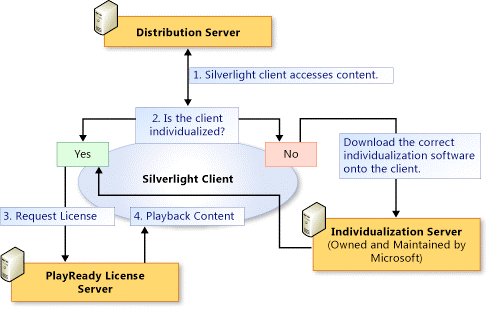
\includegraphics[height=9cm]{Figuras/autenticacao_conteudo_individualization.png} 
\label{figura:individualization}
\end{figure}
Ap\'os \textbf{\textit{License Acquisition}} o \textit{player} est\'a apto a tocar o conte\'udo. A comunica\c{c}\~ao agora \'e feita somente com o servidor de conte\'udo. Recebendo o conte\'udo criptografado e tocando atrav\'es do processo de \textbf{\textit{License Acquisition}}.
\section{\emph{Digital Right Management}}
\textcolor{red}{ Falar sobre digital Right Management e PRINCIPALMENTE SOBRE QUAIS PROBLEMAS EM AUTENTICACAO existem}

\section{Considerações Finais}
\chapter{Recifragem por \emph{Proxy}}
Nesse capítulo iremos detalhar a respeito de recifragem por \emph{proxy} (\emph{Proxy ReEncryptation} - PRE), um esquema que permite a utilização de chaves privadas de multiplos usuários para decifrar uma mensagem cifrada por um usuário \emph{u}1 sem ser necessário recifrar essa a cada vez que um usuário diferente for utilizar a mesma. Na sessão \ref{recifragem:fundamentos} irão ser apresentados os principais fundamentos da recifragem por \emph{proxy}.

% A seção \ref{recifragem:EU-PRE} irá falar sobre o \emph{Efficient Unidirectional Proxy Re-Encryption}, um esquema de recifragem por \emph{proxy} no qual é baseado a otimização proposta em \ref{recifragem:otimizacao}.


\section{Fundamentos}
\label{recifragem:fundamentos}
A recifragem por \emph{proxy} [\cite{blaze1998divertible}] é uma alternativa ao esquema criptográfico assimétrico tradicional [\cite{1363std}] que permite a delegação de direitos de acesso a messagens cifradas de maneira eficiente e mais segura. Em um cenário tradicional caso o usuário \emph{u}1 queira que somente os usuários \emph{u}2 e \emph{u}3 tenham acesso a suas mensagens cifradas ele primeiro cifra suas mensagens com sua chave privada (\emph{sk}1), em seguida cifra novamente com as chaves de \emph{u}2 e \emph{u}3 separadamente, de forma que ao distribuir essa mensagem cada um com suas respectivas chaves privadas e a chave pública de \emph{u}1 poderá decifrar a mensagem.

Em cenários onde se tem uma certa volatilidade quanto aos usuários e que a mensagem a ser transmitida não altera com tanta frequência, ou seja, existe mais mudanças de usuários que do conteúdo da mensagem. A abordagem tradicional de criptografia assimétrica se mostra uma abordagem pouco eficiente, visto que para cada vez que um usuário diferente necessitar consumir o conteúdo será necessário recifrar a mensagem a ser transmitida usando sua respectiva chave pública (\emph{pk}n) de forma que somente ele consiga reproduzi-la. Uma outra abordagem possível é através da entrega da chave privada de \emph{u}1 à \emph{u}n [\cite{ma2009group}]. Porém essa abodargem apresenta grande desvantagem visto que \emph{u}n terá acesso a chave privada de \emph{u}1 e por consequência terá acesso a todas as suas mensagens e por isso deve ser uma entidade confiável de \emph{u}1[\cite{libert2011unidirectional}].

A recifragem por \emph{proxy} explora as adptações do modelo tradicional introduzindo um novo elemento, o \emph{proxy}, que será responsável por intermediar a validação de chaves entre o usuário \emph{u}1 e seus consumidores. Simplificando é como se o \emph{proxy} agora fosse o responsável por fornecer as chaves de acesso ao conteúdo gerado por \emph{u}1 sem que o mesmo precise fornecer sua chave privada ou mesmo ter que recifrar todo o conteúdo com a chave pública dos usuários que irão consumir o mesmo.

Neste sistema o usuário \emph{u}1 irá cifrar seu conteúdo uma vez e o enviará para o \emph{proxy}. Paralelamente será gerado uma chave de recifragem que também será enviada ao \emph{proxy}. Dentro deste o conteúdo será recifrado utilizando agora a chave de recifragem de \emph{u}1 para \emph{u}n. Essa chave de recifragem permitirá ao usuário \emph{u}n decifrar o conteúdo recifrado pelo \emph{proxy} com a sua respectiva chave privada (\emph{pk}n) confome podemos observar na figura:
\begin{figure}[H]
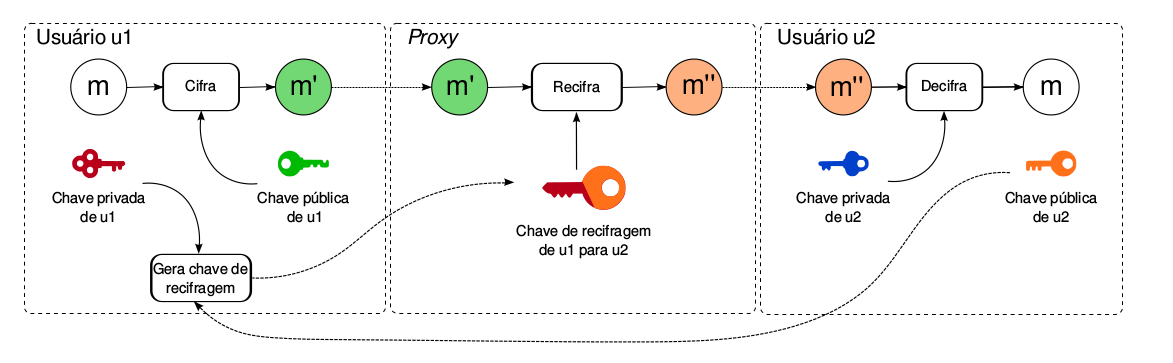
\includegraphics[width=17cm]{Figuras/recifragemPorProxy.png}
\caption{Recifragem por \emph{proxy} (\cite{mannes2016controle})} 
\label{figura:RecifragemProxy} 
\end{figure}

Há algumas premissas de operações padrão do esquemas de recifragem por \emph{proxy}. A implementação dos mesmos vai depender do tipo de recifragem[\cite{ateniese2006improved}, \cite{chow2010efficient}]:

\textbf{\textit{Configuração:}} Recebe como entrada um parâmetro de segurança $k$ e tem como saída uma tupla de parâmetros globais. 

\textbf{\textit{Geração de chaves:}} Gera os pares de chaves pública, $pk$, e privada, $sk$.

\textbf{\textit{Cifragem:}} Recebe $pk_{(u1)}$ e uma mensagem $m$, gera uma mensagem $\{m\}_{pk_{(u1)}}$.

\textbf{\textit{Geração de chave de recifragem:}} Tem como entrada a chave privada $sk_{(u1)}$ e a chave pública $pk_{(u2)}$ e como saída uma chave de recifragem $rk_{u1 \rightarrow u2}$.

\textbf{\textit{Recifragem:}} Recebe a chave de recifragem $rk_{u1 \rightarrow u2}$ e o texto cifrado $\{m\}_{pk_{(u1)}}$ , tem como saída $\{m\}_{pk_{(u2)}}$.

\textbf{\textit{Decifragem:}} Utilizando $sk_{(u2)}$ e $\{m\}_{pk_{(u2)}}$, gera como saída a mensagem $m$.

Afim de que o método seja considerado seguro foram incorporado diversas propriedades que respeitam 3 asserções básicas: (1) o \emph{proxy} não pode ser capaz de acessar o conteúdo da mensagem que recifra; (2) o usuário \emph{u}2 não pode obter o conteúdo da mensagem sem a interveção da função de recifragem; (3) O \emph{proxy} não pode, em hipótese nenhuma, obter as chaves privadas em posse das chave de recifragem e da mensagem cifrada[\cite{matsuo2007proxy},\cite{zhu2010new}].

Um resumo das possíveis caractéristicas de uma recifragem por \emph{proxy} está definido na tabela.

% ######## init table ########
%\input{2-fundam/Recifragem/fundamentos/table.tex}

A recifragem por \emph{proxy} gerou então diversas abordagens com combinações mistas de propriedades. Dentro dessas abordagens está \emph{Efficient Unidirectional Proxy Re-Encryption} (EU-PRE) [\cite{chow2010efficient}] que contempla as seguintes propriedades: (1) \textit{Unirediconal}, (2) \textit{Único salto}, (3) \textit{Intrasitivo}, (4) \textit{Interativo} e (5) \textit{Robusto contra coluio}.

Outros duas abordagens também se encaixam nessas mesmas propriedades: são elas o esquema de \emph{proxy} invisível[\cite{jia2010cca}] e o esquema de \emph{proxy} anônimo [\cite{shao2012anonymous}]. Dessas três abordagens o EU-PRE se mostra mais simples e eficente, pois não implementa as funções de anonimato das mensagens cifradas e nem as funções de invisibilidade do \emph{proxy}.

Além disso, o trabalho de \cite{mannes2016controle} apresenta uma nova abordagem quanto ao EU-PRE. Retirando do sistema a necessidade de ter um agente de \emph{proxy}  sem impactar na segurança do processo.

Esse processo é feito através da otimização das equações matemáticas onde o processo de cifragem ainda ficará com o provedor de conteúdo e os de decifragem e recifragem ficarão a cargo do usuário. Eliminando assim um terceiro elemento do sistema, o que torna-o muito mais parecido com os que temos hoje.
%\section{\emph{Efficient Unidirectional Proxy Re-Encryptation}}
\label{recifragem:EU-PRE}
O \emph{Efficient Unidirectional Proxy Re-Encryptation}, o qual a partir daqui o iremos referenciá-lo com EU-PRE, possui seis algoritmos principais: \emph{configuração},\emph{geração de chaves}, \emph{cifragem},\emph{geração de chave de recifragem}, \emph{recifragem} e \emph{decifragem}. Que são detalhados, segundo \cite{mannes2016controle}, como os seguintes:

\paragraph{Configuração:} escolher dois números primos \emph{p} e \emph{q} tal que \emph{q} | \emph{p} - 1 (\emph{q} deve ser divisor de (p-1)), o parâmetro $\ell_0$ para o tamanho da mensagem, o parâmetro de segurança $\ell_1$ e um gerador \emph{g} do grupo $\mathbb{G}$ (um subgrupo de $\mathbb{Z^*_q}$ de ordem $q$). Além desses parâmetros, o sistema utiliza quatro funções de $hash$:$H_1 : {\left\{0,1\right\}}^{\ell_0} \times {\left\{0,1\right\}}^{\ell_1} \rightarrow \mathbb{Z^*_q}$, $H_2: \mathbb{G} \rightarrow {\left\{0,1\right\}}^{\ell_0 + \ell_1}$, $H_3 : {\left\{0,1\right\}}^{*} \rightarrow \mathbb{Z^*_q}$, $H_4 :  \mathbb{G} \rightarrow \mathbb{Z^*_q}$ . Os parâmetros públicos do sistema são: $\left(\emph{q},\mathbb{G},\emph{g},H_1,H_2,H_3,H_4,\ell_0,\ell_1\right)$.

\paragraph{Geração de chaves:} O conjunto de chaves do EU-PRE é composto por dois pares de chaves públicas-privadas para cada usuário do sistema. Essa caracaterística é introduzida por \cite{chow2010efficient} para garantir que a chave privada de um usuário \emph{u}1 não seja divulgada caso o \emph{proxy} e o usuário troquem informações. Considerando um usuário \emph{u}1, as chaves privadas $\emph{sk}1_{(\emph{u}1)}$ e $\emph{sk}2_{(\emph{u}1)}$ são escolhidas aleatoriamente em $\mathbb{Z}^*_q$ e as chaves públicas são calculadas por $\emph{g}^{sk}$, assim $sk1_{\emph({u}1)}$ = $\emph{g}^{sk_{(\emph{u}1)}}\mod{p}$ e $pk2_{(u1)} = \emph{g}^{(sk1)}\mod{p}$.   

\paragraph{Cifragem:} uma mensagem $m$ é cifrada pelo usuário $u1$
com suas chaves públicas $pk1_{(u1)}$ e $pk2_{(u1)}$. Escolher $t$ a partir de $\mathbb{Z}^*_q$ e $\omega$ de tamanho $\ell_1$ e calcular $r = H_1(m,\omega)$ e $D,E$ e $F$ como segue:
\begin{equation}
    D = ({{pk1^{H_{4(pk2_{u1})}}_{(u1)}} \times pk2_{(u1)})}^t \mod{p} )
\end{equation}
\begin{equation}
    E = ({pk1^{H_{4(pk2_{(u1)})}} \times pk2_{u1} })^r\mod{p})
\end{equation}
\begin{equation}
    F = H_2(g^r\mod{p})\oplus(m\parallel \omega) 
\end{equation}

Calcular também $ r = t+r\bullet H_3(D,E,F)\mod{p}$. A saída é $(D,F,E,s)$
\paragraph{Geração de chaves de recifragem:} Para geração de chave de recifragem de $u1$ para $u2$, são necessárias as chaves privadas de $u1$ e uma das chaves públicas de $u2$,$pk2_{(u2)}$. Deve-se escolher aleatoriamente $h$ de tamanho $\ell_0$ e $\pi$ de tamanho $\ell_1$ e calcular $v = H_1(h \times \pi)$. Calcular também $V = pk2^v_{(u2)} \mod{p}$ e $W = H_2(g^v\mod{p})\oplus(h \parallel \pi)$.
A chave de recifragem é:
\begin{equation}
    rk_{u1\rightarrow u2} = \big( {(sk1_{(u1)}) \bullet H_4(pk2_{(u2)} + sk2_{(u2)})}^{-1} \mod{p-1}  \big)
\end{equation}
A saída é $(rk_{u1\rightarrow u2},V,W)$.

\paragraph{Recifragem:}
Primeiramente o \emph{proxy} deve verificar :
\begin{equation}
\label{equation:rk}
    {(pk1^{H4(pk2_{(u1)})}_{(u1)} \bullet {pk2_{(u1)}\mod{p}})}^s \mod{p} = D \bullet (E^{H_3(D,E,F)} \mod{p} )\mod{p}
\end{equation}
E caso a equação \ref{equation:rk} seja verdadeira:
\begin{equation}
\label{equation:eu-pre:recifragem}
    E' = E^{rk_{u1\rightarrow u2}} \mod{p}
\end{equation}
A saída será $(E',F,V,W)$.
\paragraph{Decifragem:} A mensagem $m$ é decifrada por $u2$ mediante sua chave privada $sk2_{(u2)}$.
Primeiramente o usuário $u2$ recupera $(h\parallel\pi)$ e $(m\parallel\omega)$ ao calcular:
\begin{equation}
    (h\parallel\pi) = W \oplus H_2(V^{sk^{-1}_{(u2)}\mod{p-1}} \mod{p})
\end{equation}
\begin{equation}
\label{equation:eu-pre:decifragem}
    (m\parallel\omega) = F \oplus H_2(E'^{h^{-1}\mod{p-1}} \mod{p})
\end{equation}
A saída é a mensagem $m$ se $V = {pk2^{H_1(h,\pi)}_{(u2)}} \mod{p}$ e $E' = g^{H_1(m,\omega)\bullet h} \mod{p}$.
Na figura \ref{figura:fluxo_eu-pre} podemos visualizar todo o processo de recifragem do EU-PRE e o fluxo sequencial de cada etapa.
\begin{figure}[H]
\caption{Fluxo de processos do EU-PRE (\cite{mannes2016controle})
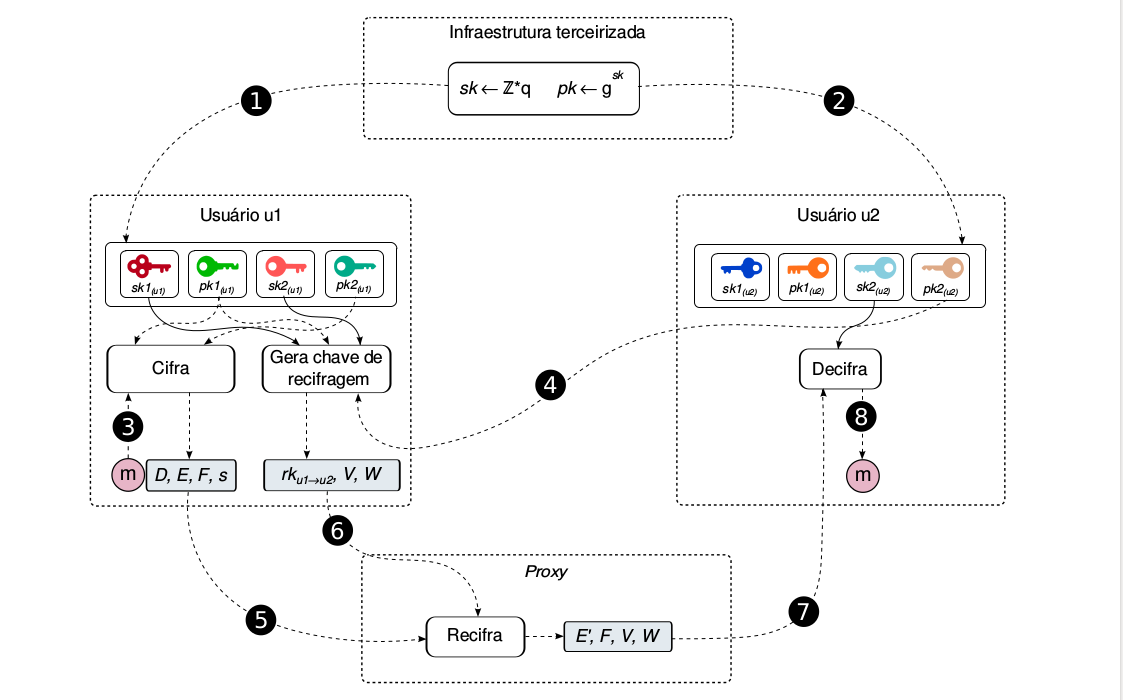
\includegraphics[height=11cm]{Figuras/fluxo_EU-PRE.png} 
\label{figura:fluxo_eu-pre}
\end{figure}

É importante salientar que no esquema de recifragrem por \emph{proxy} tradicionalmente é composto por quatro entidades: uma infraestrutura terceirizada responsável por delegar as chaves que serão utilizadas, o usuário que as delega, o \emph{proxy} e o usuário que recebe e delegação. 
Dentro desse ecosistema a divisão: Os algoritmos de configuração e geração de chaves dos usuários são executados na infraestrutura terceirizada. A cifragem e a geração de chaves de cifragem são realizadas no usuário que delega os direitos de recifragem. A recifragem é responsabilidade do \emph{proxy} e a decifragem é executada no usuário (dispositivo) que irá consumir as informações.
%\section{Otimização do \textbf{EU-PRE}}
\label{recifragem:otimizacao}
No trabalho de \cite{mannes2016controle} propõe-se uma otimização do processo do EU-PRE (\ref{recifragem:EU-PRE}). A otimizição envolve as equações \ref{equation:eu-pre:recifragem}(Recifragem) e \ref{equation:eu-pre:decifragem}(Decifragem). No modelo tradicional o \emph{proxy} recebe do provedor as variáveis $(D,E,F,s)$ e a chave de recifragem $(rk_{c\rightarrow u},V,W)$ do conteúdo $c$ para o usuário $u$. E, após a validação com as variáveis $D$ e $E$ é inciado o processo de recifragem para o $u$ através da equação \ref{equation:eu-pre:decifra}.E assim, o \emph{proxy} envia ao usuário $u$ as informações $(E',F,V,W)$ onde $E'$ é a variável calculada na equação anterior. E assim, como visto na equação \ref{equation:eu-pre:recuperaConteudo}, recupera o conteúdo cifrado pelo provedor.
\begin{equation}
\label{equation:eu-pre:decifra}
    E' = E^{rk_{c\rightarrow u}}\mod{p}
\end{equation}
\begin{equation}
\label{equation:eu-pre:recuperaConteudo}
    (m\parallel \omega) = F \oplus H_2({E'}^{h^{-1}\mod{p-1}} \mod{p})
\end{equation}
No trabalho é apresentado uma proposta de que essas duas operações sejam realizadas na mesma entidade, simplificando assim o processo de recifragem. Onde o usuário recebe o conteúdo diretamente do provedor. Essa operação é feita aplicando a variável $E$ diretamente na equação \ref{equation:eu-pre:decifra}. Eliminando a equação \ref{equation:eu-pre:decifra} ao substituir o $E'$ recebido do \emph{proxy}. Como podemos ver em \ref{equation:eu-pre:otimizacao}.
\begin{equation} \label{equation:eu-pre:otimizacao}
    \begin{split}
        (m\parallel \omega) & = F \oplus H_2({({E}^{rk_{c\rightarrow u}})^{\frac{1}{h}\mod{p-1}}} \mod{p}) \\
 & = F \oplus H_2({({E}^{rk_{c\rightarrow u{\frac{1}{h}\mod{p-1}}}})} \mod{p}) \\
 & = F \oplus H_2({({E}^{{\frac{rk_{c\rightarrow u}}{h}\mod{p-1}}})} \mod{p})
    \end{split}
\end{equation}

Com a equação final visualizada em \ref{equation:eu-pre:otimizacao} podemos ter um processo de recifragem por \emph{proxy} que possui no máximo o envolvimento de três entidades: o usuário, o provedor e uma infraestrutura responsável por delegar as chaves.

A infraestura responsável por delegar as chaves pode ainda ser substituída/rodada no provedor do conteúdo simplificando ainda mais as entidades envolvidas para duas: o provedor e o usuário consumidor.


\section{Considerações Finais}

Nesse capítulo vimos por linhas gerais o esquema de criptografia conhecido como recifragem por \emph{proxy}. Vimos também um método de otimização do mesmo que possibilita a retirada do servidor de \emph{proxy} sem perder a segurança e a característica principal do processo que é permitir que o conteúdo seja cifrado uma vez por $u1$ e decifrado por $n$ usuários sem que o mesmo tenha que cifrar novamente para esses $n$ usuários com suas respectivas chaves.

Toda essa proposta pode se encaixar dentro de um ambiente de CDN. Facilitando que o conteúdo seja retrasmitido pela rede, ficando em vários servidores de ponta e estejam devidamente criptografados. E mesmo que essa base de usuários mude,como é o caso de fornecedoras de VOD, esse conteúdo não precisa ser novamente recifrado.		% fundamentação teórica
%\section{Fundamentos}
\label{recifragem:fundamentos}
A recifragem por \emph{proxy} [\cite{blaze1998divertible}] é uma alternativa ao esquema criptográfico assimétrico tradicional [\cite{1363std}] que permite a delegação de direitos de acesso a messagens cifradas de maneira eficiente e mais segura. Em um cenário tradicional caso o usuário \emph{u}1 queira que somente os usuários \emph{u}2 e \emph{u}3 tenham acesso a suas mensagens cifradas ele primeiro cifra suas mensagens com sua chave privada (\emph{sk}1), em seguida cifra novamente com as chaves de \emph{u}2 e \emph{u}3 separadamente, de forma que ao distribuir essa mensagem cada um com suas respectivas chaves privadas e a chave pública de \emph{u}1 poderá decifrar a mensagem.

Em cenários onde se tem uma certa volatilidade quanto aos usuários e que a mensagem a ser transmitida não altera com tanta frequência, ou seja, existe mais mudanças de usuários que do conteúdo da mensagem. A abordagem tradicional de criptografia assimétrica se mostra uma abordagem pouco eficiente, visto que para cada vez que um usuário diferente necessitar consumir o conteúdo será necessário recifrar a mensagem a ser transmitida usando sua respectiva chave pública (\emph{pk}n) de forma que somente ele consiga reproduzi-la. Uma outra abordagem possível é através da entrega da chave privada de \emph{u}1 à \emph{u}n [\cite{ma2009group}]. Porém essa abodargem apresenta grande desvantagem visto que \emph{u}n terá acesso a chave privada de \emph{u}1 e por consequência terá acesso a todas as suas mensagens e por isso deve ser uma entidade confiável de \emph{u}1[\cite{libert2011unidirectional}].

A recifragem por \emph{proxy} explora as adptações do modelo tradicional introduzindo um novo elemento, o \emph{proxy}, que será responsável por intermediar a validação de chaves entre o usuário \emph{u}1 e seus consumidores. Simplificando é como se o \emph{proxy} agora fosse o responsável por fornecer as chaves de acesso ao conteúdo gerado por \emph{u}1 sem que o mesmo precise fornecer sua chave privada ou mesmo ter que recifrar todo o conteúdo com a chave pública dos usuários que irão consumir o mesmo.

Neste sistema o usuário \emph{u}1 irá cifrar seu conteúdo uma vez e o enviará para o \emph{proxy}. Paralelamente será gerado uma chave de recifragem que também será enviada ao \emph{proxy}. Dentro deste o conteúdo será recifrado utilizando agora a chave de recifragem de \emph{u}1 para \emph{u}n. Essa chave de recifragem permitirá ao usuário \emph{u}n decifrar o conteúdo recifrado pelo \emph{proxy} com a sua respectiva chave privada (\emph{pk}n) confome podemos observar na figura:
\begin{figure}[H]
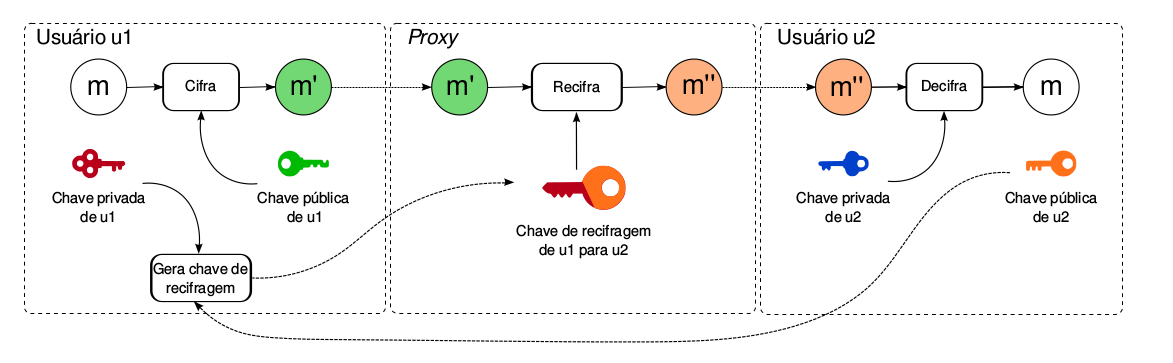
\includegraphics[width=17cm]{Figuras/recifragemPorProxy.png}
\caption{Recifragem por \emph{proxy} (\cite{mannes2016controle})} 
\label{figura:RecifragemProxy} 
\end{figure}

Há algumas premissas de operações padrão do esquemas de recifragem por \emph{proxy}. A implementação dos mesmos vai depender do tipo de recifragem[\cite{ateniese2006improved}, \cite{chow2010efficient}]:

\textbf{\textit{Configuração:}} Recebe como entrada um parâmetro de segurança $k$ e tem como saída uma tupla de parâmetros globais. 

\textbf{\textit{Geração de chaves:}} Gera os pares de chaves pública, $pk$, e privada, $sk$.

\textbf{\textit{Cifragem:}} Recebe $pk_{(u1)}$ e uma mensagem $m$, gera uma mensagem $\{m\}_{pk_{(u1)}}$.

\textbf{\textit{Geração de chave de recifragem:}} Tem como entrada a chave privada $sk_{(u1)}$ e a chave pública $pk_{(u2)}$ e como saída uma chave de recifragem $rk_{u1 \rightarrow u2}$.

\textbf{\textit{Recifragem:}} Recebe a chave de recifragem $rk_{u1 \rightarrow u2}$ e o texto cifrado $\{m\}_{pk_{(u1)}}$ , tem como saída $\{m\}_{pk_{(u2)}}$.

\textbf{\textit{Decifragem:}} Utilizando $sk_{(u2)}$ e $\{m\}_{pk_{(u2)}}$, gera como saída a mensagem $m$.

Afim de que o método seja considerado seguro foram incorporado diversas propriedades que respeitam 3 asserções básicas: (1) o \emph{proxy} não pode ser capaz de acessar o conteúdo da mensagem que recifra; (2) o usuário \emph{u}2 não pode obter o conteúdo da mensagem sem a interveção da função de recifragem; (3) O \emph{proxy} não pode, em hipótese nenhuma, obter as chaves privadas em posse das chave de recifragem e da mensagem cifrada[\cite{matsuo2007proxy},\cite{zhu2010new}].

Um resumo das possíveis caractéristicas de uma recifragem por \emph{proxy} está definido na tabela.

% ######## init table ########
%% ######## init table ########

\begin{table}[!htp]
\begin{tabular}{|c|c|c|}
\hline
Propriedades & Valores & Descrição \\ \hline
\multirow{Direção da delegação} & Unidirecional  & a  delegação $u1 \rightarrow u2$ não implica na delegação de $u2 \rightarrow u1$ \\ \cline{2-2}\cline{3-3} 
& Bidirecional  & a delegação u1 → u2 implica na delegação de u2 → u1 \\ \hline

\multirow{Número de saltos de recifragrem} & Único Salto \centering & somente mensagens originais podem ser recifradas \\ \cline{2-2}\cline{3-3} 
& Multiplos Saltos \centering & uma mensagem recifrada de u1 → u2 pode ser novamente recifrada de u2 → u3 \\ \hline

\multirow{Transitividade da chave de recifragem} & Transitivo & descrição transitivo \\ \cline{2-2}\cline{3-3} 
& Intransitivo \centering & o proxy não pode, a partir de rk u1→u2 e rk u2→u3 ,produzir rk u1→u3 \\ \hline

\multirow{Necessidade de iteração com o usuário} & Iterativo \centering & as chaves de recifragem são geradas por u1 com a necessidade de interações com u2 \\ \cline{2-2}\cline{3-3} 
& Não iterativo \centering & as chaves de recifragem são geradas por u1 sem a necessidade de interações com u2 \\ \hline

\multirow{Robustez contra conluio} & Robusto \centering & o usuário u2 e o proxy em conluio não conseguem recuperar a chave privada de u1 \\ \cline{2-2}\cline{3-3} 
& Não robusto \centering & o usuário u2 e o proxy em conluio conseguem recuperar a chave privada de u1 \\ \hline
\end{tabular}
\caption{Propriedades dos esquemas de recifragem por \textit{proxy}}
\label{table}
\end{table}

A recifragem por \emph{proxy} gerou então diversas abordagens com combinações mistas de propriedades. Dentro dessas abordagens está \emph{Efficient Unidirectional Proxy Re-Encryption} (EU-PRE) [\cite{chow2010efficient}] que contempla as seguintes propriedades: (1) \textit{Unirediconal}, (2) \textit{Único salto}, (3) \textit{Intrasitivo}, (4) \textit{Interativo} e (5) \textit{Robusto contra coluio}.

Outros duas abordagens também se encaixam nessas mesmas propriedades: são elas o esquema de \emph{proxy} invisível[\cite{jia2010cca}] e o esquema de \emph{proxy} anônimo [\cite{shao2012anonymous}]. Dessas três abordagens o EU-PRE se mostra mais simples e eficente, pois não implementa as funções de anonimato das mensagens cifradas e nem as funções de invisibilidade do \emph{proxy}.

Além disso, o trabalho de \cite{mannes2016controle} apresenta uma nova abordagem quanto ao EU-PRE. Retirando do sistema a necessidade de ter um agente de \emph{proxy}  sem impactar na segurança do processo.

Esse processo é feito através da otimização das equações matemáticas onde o processo de cifragem ainda ficará com o provedor de conteúdo e os de decifragem e recifragem ficarão a cargo do usuário. Eliminando assim um terceiro elemento do sistema, o que torna-o muito mais parecido com os que temos hoje.		% revisão bibliográfica (estado da arte)
\chapter{Controle de acesso em CDN utilizando recifragem por \emph{proxy}}

\section{Contextualização}
\label{proposta:justificativa}
Com a demanda crescente da necessidade de conteúdo \emph{On-Demand} de áudio e vídeo através das plataformas de serviços de \emph{streaming} como \emph{Netflix}, \emph{Amazon Video Prime}, \emph{Spotify}, \emph{Deezer} e tantas outras que vem surgindo cada dia. Somado ao fato de que todas esses serviços estão ligados diretamente a algum tipo de serviço de CDN, pois todos estão em escala global mas absorvem particularidades locais de cada parte do mundo onde se encontram disponíveis. 

É necessário que haja um processo de criptografia que possa ser menos custoso, ou seja, que faça menos requisições de chaves, quando comparado a outros métodos, pra evitar o máximo possível tráfego de informações na rede, e que permita a volatilidade de base de usuários que esses serviços tem, sem ter que se preocupar  com recifragem do conteúdo para cada usuário que sai/entra dentro do banco de serviços.

Com isso, a proposta de recifragem por \emph{proxy}, se utilizada dentro de um ambiente de CDN, pode trazer benefícios à serviços como esse. Levaremos em conta as otimizações apresentada por \cite{mannes2016controle} que considera a supressão da entidade \emph{proxy} do sistema passando o processo de recifragem para o usuário que acumulará com o processo de decifragem.

Ainda será necessário a presença do provedor cifrando o conteúdo transmitido. Mas essa cifragem ainda será feita apenas uma vez e a recifragens e decifragens necessárias serão feitas pelos $n$ que requisitarem o conteúdo.  

O trabalho de \cite{mannes2016controle} segue uma abordagem muito semelhante mas aplica esses conceitos em um outro tipo de ambiente, o de Redes Centradas em Informações [\cite{redesCentradasInfo}].
\section{Proposta}
\label{proposta:metodologia}
O objetivo principal da pesquisa é aplicar a otimização do EU-PRE dentro de um ambiente CDN validando-o através de um ambiente de simulação pré-existente.

Será utilizado o simulador desenvolvido por \cite{stamos2010cdnsim} como base para aplicação de protocolos de CDN. Modificando-o, com a devida autorização dos criadores, em alguns pontos específicos que estão relacionados ao processo de criptografia. Verificando primeiro se já existe algum tipo de criptografia dentro do simulador para possíveis comparações futuras.
Caso não haja nenhum será desenvolvido primeiro a proposta apresentada comparando-o com os valores sem criptografia para verificar o impacto do mesmo em situações desprotegidas.

Para desenvolver a proposta são necessários os seguintes passos:
\begin{enumerate}

    \item \label{proposta:EstudoCDN} Estudo sobre CDN e as soluções de controle de acesso utilizadas;
    \item \label{proposta:EstudoRecifragem} Estudo de recifragem de \emph{proxy}.
    \item \label{proposta:AnaliseSim} Ánalise dos simuladores de CDN disponíveis e escolha de um deles;
    \item \label{proposta:Atualizacao} Atualização (necessária) do simulador apresentado por \cite{stamos2010cdnsim} para versões mais recentes do OMNet++ [OMNet++];
    \item \label{proposta:ValidacaoProcesso} Validação de processos criptográficos já existentes dentro do simulador;
    \item \label{proposta:Desenvolvimento} Desenvolvimento do processo de recifragem por \emph{proxy} dentro do simulador;
    \item \label{proposta:DefExperimentos} Definição de experimentos para validação da proposta;
    \item \label{proposta:ValidacaoProposta} Validação da proposta;
    \item \label{proposta:Publicacao} Publicação de resultados.

\end{enumerate}

\definecolor{STC}{rgb}{0,1,0}
\begin{table}[!htbp]
    \centering
    \begin{tabular}{|c|c|c|c|c|c|c|c|c|c|c|c|c|}
    \hline
    & \multicolumn{7}{c|}{2018}&\multicolumn{5}{c|}{2019} \\
    \hline
    & JUN&JUL&AGO&SET&OUT&NOV&DEZ&JAN&FEV&MAR&ABR&JUN \\
    \hline
    \ref{proposta:EstudoCDN}&\cellcolor{STC}&\cellcolor{STC}&&&&&&&&&& \\
    \hline
    \ref{proposta:EstudoRecifragem} &&&\cellcolor{STC}&\cellcolor{STC}&&&&&&&& \\
    \hline
    \ref{proposta:AnaliseSim} &&&&&\cellcolor{STC}&&&&&&& \\
    \hline
    \ref{proposta:Atualizacao} &&&&&&\cellcolor{STC}&\cellcolor{STC}&&&&& \\
    \hline
    \ref{proposta:ValidacaoProcesso} &&&&&&&&\cellcolor{STC}&&&& \\
    \hline
    \ref{proposta:Desenvolvimento} &&&&&&&&\cellcolor{STC}&\cellcolor{STC}&&& \\
    \hline
    \ref{proposta:DefExperimentos} &&&&&&&&&&\cellcolor{STC}&& \\
    \hline
    \ref{proposta:ValidacaoProposta} &&&&&&&&&&\cellcolor{STC}&& \\
    \hline
    \ref{proposta:Publicacao} &&&&&&&&&&&\cellcolor{STC}&\cellcolor{STC} \\
    \hline
    \end{tabular}
    \caption{Cronograma}
    \label{tab:cronograma}
\end{table}


Todo o processo será desenvolvido utilizando Python e C/C++ que são as linguagem aplicadas dentro do simulador [\cite{stamos2010cdnsim}].
\section{Resultados esperados}
\label{proposta:resultadosEsperados}
Caso já tenha processos de criptografia implementado são esperados que os valores obitdos tenham melhoras significativas, ou no mínimo semelhantes, a processos já existentes. Muito semelhante ao impacto obtido por \cite{mannes2016controle} para Redes Centradas em Informações [\cite{redesCentradasInfo}].

E caso não haja esses processos, então, é esperado que o impacto da criptografia seja mínimo quanto quando comparado com sem criptografia. 

\section{Considerações Finais}
		% proposta
%\section{Fundamentos}
\label{recifragem:fundamentos}
A recifragem por \emph{proxy} [\cite{blaze1998divertible}] é uma alternativa ao esquema criptográfico assimétrico tradicional [\cite{1363std}] que permite a delegação de direitos de acesso a messagens cifradas de maneira eficiente e mais segura. Em um cenário tradicional caso o usuário \emph{u}1 queira que somente os usuários \emph{u}2 e \emph{u}3 tenham acesso a suas mensagens cifradas ele primeiro cifra suas mensagens com sua chave privada (\emph{sk}1), em seguida cifra novamente com as chaves de \emph{u}2 e \emph{u}3 separadamente, de forma que ao distribuir essa mensagem cada um com suas respectivas chaves privadas e a chave pública de \emph{u}1 poderá decifrar a mensagem.

Em cenários onde se tem uma certa volatilidade quanto aos usuários e que a mensagem a ser transmitida não altera com tanta frequência, ou seja, existe mais mudanças de usuários que do conteúdo da mensagem. A abordagem tradicional de criptografia assimétrica se mostra uma abordagem pouco eficiente, visto que para cada vez que um usuário diferente necessitar consumir o conteúdo será necessário recifrar a mensagem a ser transmitida usando sua respectiva chave pública (\emph{pk}n) de forma que somente ele consiga reproduzi-la. Uma outra abordagem possível é através da entrega da chave privada de \emph{u}1 à \emph{u}n [\cite{ma2009group}]. Porém essa abodargem apresenta grande desvantagem visto que \emph{u}n terá acesso a chave privada de \emph{u}1 e por consequência terá acesso a todas as suas mensagens e por isso deve ser uma entidade confiável de \emph{u}1[\cite{libert2011unidirectional}].

A recifragem por \emph{proxy} explora as adptações do modelo tradicional introduzindo um novo elemento, o \emph{proxy}, que será responsável por intermediar a validação de chaves entre o usuário \emph{u}1 e seus consumidores. Simplificando é como se o \emph{proxy} agora fosse o responsável por fornecer as chaves de acesso ao conteúdo gerado por \emph{u}1 sem que o mesmo precise fornecer sua chave privada ou mesmo ter que recifrar todo o conteúdo com a chave pública dos usuários que irão consumir o mesmo.

Neste sistema o usuário \emph{u}1 irá cifrar seu conteúdo uma vez e o enviará para o \emph{proxy}. Paralelamente será gerado uma chave de recifragem que também será enviada ao \emph{proxy}. Dentro deste o conteúdo será recifrado utilizando agora a chave de recifragem de \emph{u}1 para \emph{u}n. Essa chave de recifragem permitirá ao usuário \emph{u}n decifrar o conteúdo recifrado pelo \emph{proxy} com a sua respectiva chave privada (\emph{pk}n) confome podemos observar na figura:
\begin{figure}[H]
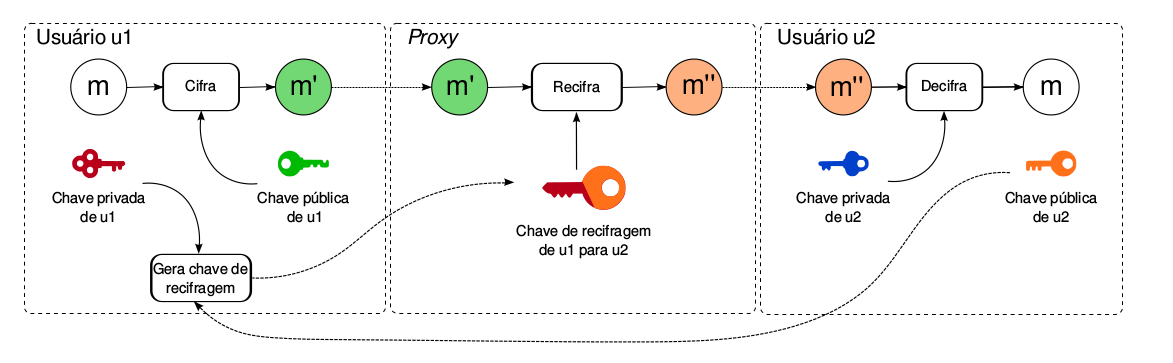
\includegraphics[width=17cm]{Figuras/recifragemPorProxy.png}
\caption{Recifragem por \emph{proxy} (\cite{mannes2016controle})} 
\label{figura:RecifragemProxy} 
\end{figure}

Há algumas premissas de operações padrão do esquemas de recifragem por \emph{proxy}. A implementação dos mesmos vai depender do tipo de recifragem[\cite{ateniese2006improved}, \cite{chow2010efficient}]:

\textbf{\textit{Configuração:}} Recebe como entrada um parâmetro de segurança $k$ e tem como saída uma tupla de parâmetros globais. 

\textbf{\textit{Geração de chaves:}} Gera os pares de chaves pública, $pk$, e privada, $sk$.

\textbf{\textit{Cifragem:}} Recebe $pk_{(u1)}$ e uma mensagem $m$, gera uma mensagem $\{m\}_{pk_{(u1)}}$.

\textbf{\textit{Geração de chave de recifragem:}} Tem como entrada a chave privada $sk_{(u1)}$ e a chave pública $pk_{(u2)}$ e como saída uma chave de recifragem $rk_{u1 \rightarrow u2}$.

\textbf{\textit{Recifragem:}} Recebe a chave de recifragem $rk_{u1 \rightarrow u2}$ e o texto cifrado $\{m\}_{pk_{(u1)}}$ , tem como saída $\{m\}_{pk_{(u2)}}$.

\textbf{\textit{Decifragem:}} Utilizando $sk_{(u2)}$ e $\{m\}_{pk_{(u2)}}$, gera como saída a mensagem $m$.

Afim de que o método seja considerado seguro foram incorporado diversas propriedades que respeitam 3 asserções básicas: (1) o \emph{proxy} não pode ser capaz de acessar o conteúdo da mensagem que recifra; (2) o usuário \emph{u}2 não pode obter o conteúdo da mensagem sem a interveção da função de recifragem; (3) O \emph{proxy} não pode, em hipótese nenhuma, obter as chaves privadas em posse das chave de recifragem e da mensagem cifrada[\cite{matsuo2007proxy},\cite{zhu2010new}].

Um resumo das possíveis caractéristicas de uma recifragem por \emph{proxy} está definido na tabela.

% ######## init table ########
%% ######## init table ########

\begin{table}[!htp]
\begin{tabular}{|c|c|c|}
\hline
Propriedades & Valores & Descrição \\ \hline
\multirow{Direção da delegação} & Unidirecional  & a  delegação $u1 \rightarrow u2$ não implica na delegação de $u2 \rightarrow u1$ \\ \cline{2-2}\cline{3-3} 
& Bidirecional  & a delegação u1 → u2 implica na delegação de u2 → u1 \\ \hline

\multirow{Número de saltos de recifragrem} & Único Salto \centering & somente mensagens originais podem ser recifradas \\ \cline{2-2}\cline{3-3} 
& Multiplos Saltos \centering & uma mensagem recifrada de u1 → u2 pode ser novamente recifrada de u2 → u3 \\ \hline

\multirow{Transitividade da chave de recifragem} & Transitivo & descrição transitivo \\ \cline{2-2}\cline{3-3} 
& Intransitivo \centering & o proxy não pode, a partir de rk u1→u2 e rk u2→u3 ,produzir rk u1→u3 \\ \hline

\multirow{Necessidade de iteração com o usuário} & Iterativo \centering & as chaves de recifragem são geradas por u1 com a necessidade de interações com u2 \\ \cline{2-2}\cline{3-3} 
& Não iterativo \centering & as chaves de recifragem são geradas por u1 sem a necessidade de interações com u2 \\ \hline

\multirow{Robustez contra conluio} & Robusto \centering & o usuário u2 e o proxy em conluio não conseguem recuperar a chave privada de u1 \\ \cline{2-2}\cline{3-3} 
& Não robusto \centering & o usuário u2 e o proxy em conluio conseguem recuperar a chave privada de u1 \\ \hline
\end{tabular}
\caption{Propriedades dos esquemas de recifragem por \textit{proxy}}
\label{table}
\end{table}

A recifragem por \emph{proxy} gerou então diversas abordagens com combinações mistas de propriedades. Dentro dessas abordagens está \emph{Efficient Unidirectional Proxy Re-Encryption} (EU-PRE) [\cite{chow2010efficient}] que contempla as seguintes propriedades: (1) \textit{Unirediconal}, (2) \textit{Único salto}, (3) \textit{Intrasitivo}, (4) \textit{Interativo} e (5) \textit{Robusto contra coluio}.

Outros duas abordagens também se encaixam nessas mesmas propriedades: são elas o esquema de \emph{proxy} invisível[\cite{jia2010cca}] e o esquema de \emph{proxy} anônimo [\cite{shao2012anonymous}]. Dessas três abordagens o EU-PRE se mostra mais simples e eficente, pois não implementa as funções de anonimato das mensagens cifradas e nem as funções de invisibilidade do \emph{proxy}.

Além disso, o trabalho de \cite{mannes2016controle} apresenta uma nova abordagem quanto ao EU-PRE. Retirando do sistema a necessidade de ter um agente de \emph{proxy}  sem impactar na segurança do processo.

Esse processo é feito através da otimização das equações matemáticas onde o processo de cifragem ainda ficará com o provedor de conteúdo e os de decifragem e recifragem ficarão a cargo do usuário. Eliminando assim um terceiro elemento do sistema, o que torna-o muito mais parecido com os que temos hoje.		% experimentação e validação
\chapter{Cronograma}

\lipsum[11-14]	% texto aleatório
		% cronograma
%\chapter{Conclusão}

\lipsum[11-14]	% texto aleatório
		% conclusão

%=====================================================

% Estilos de bibliografia recomendados (só descomentar um estilo!)
% Mais infos: https://pt.sharelatex.com/learn/Bibtex_bibliography_styles
\bibliographystyle{apalike-ptbr}	% [Maziero et al., 2006]
%\bibliographystyle{alpha}		% [Maz06]
%\bibliographystyle{plainnat}		% vide Google "LaTeX Natbib"
%\bibliographystyle{plain}		% [1] ordem alfabética
%\bibliographystyle{unsrt}		% [1] ordem de uso no texto

% no estilo "unsrt", evita que citações nos índices sejam consideradas
%\usepackage{notoccite}

% base de bibliografia (BibTeX)
\bibliography{referencias}
%\bibliography{file1, file2, file3} % se tiver mais de um arquivo BibTeX

%=====================================================

% inclusão de apêndices
\appendix

% inclusão de apêndice
\section{Fundamentos}
\label{recifragem:fundamentos}
A recifragem por \emph{proxy} [\cite{blaze1998divertible}] é uma alternativa ao esquema criptográfico assimétrico tradicional [\cite{1363std}] que permite a delegação de direitos de acesso a messagens cifradas de maneira eficiente e mais segura. Em um cenário tradicional caso o usuário \emph{u}1 queira que somente os usuários \emph{u}2 e \emph{u}3 tenham acesso a suas mensagens cifradas ele primeiro cifra suas mensagens com sua chave privada (\emph{sk}1), em seguida cifra novamente com as chaves de \emph{u}2 e \emph{u}3 separadamente, de forma que ao distribuir essa mensagem cada um com suas respectivas chaves privadas e a chave pública de \emph{u}1 poderá decifrar a mensagem.

Em cenários onde se tem uma certa volatilidade quanto aos usuários e que a mensagem a ser transmitida não altera com tanta frequência, ou seja, existe mais mudanças de usuários que do conteúdo da mensagem. A abordagem tradicional de criptografia assimétrica se mostra uma abordagem pouco eficiente, visto que para cada vez que um usuário diferente necessitar consumir o conteúdo será necessário recifrar a mensagem a ser transmitida usando sua respectiva chave pública (\emph{pk}n) de forma que somente ele consiga reproduzi-la. Uma outra abordagem possível é através da entrega da chave privada de \emph{u}1 à \emph{u}n [\cite{ma2009group}]. Porém essa abodargem apresenta grande desvantagem visto que \emph{u}n terá acesso a chave privada de \emph{u}1 e por consequência terá acesso a todas as suas mensagens e por isso deve ser uma entidade confiável de \emph{u}1[\cite{libert2011unidirectional}].

A recifragem por \emph{proxy} explora as adptações do modelo tradicional introduzindo um novo elemento, o \emph{proxy}, que será responsável por intermediar a validação de chaves entre o usuário \emph{u}1 e seus consumidores. Simplificando é como se o \emph{proxy} agora fosse o responsável por fornecer as chaves de acesso ao conteúdo gerado por \emph{u}1 sem que o mesmo precise fornecer sua chave privada ou mesmo ter que recifrar todo o conteúdo com a chave pública dos usuários que irão consumir o mesmo.

Neste sistema o usuário \emph{u}1 irá cifrar seu conteúdo uma vez e o enviará para o \emph{proxy}. Paralelamente será gerado uma chave de recifragem que também será enviada ao \emph{proxy}. Dentro deste o conteúdo será recifrado utilizando agora a chave de recifragem de \emph{u}1 para \emph{u}n. Essa chave de recifragem permitirá ao usuário \emph{u}n decifrar o conteúdo recifrado pelo \emph{proxy} com a sua respectiva chave privada (\emph{pk}n) confome podemos observar na figura:
\begin{figure}[H]
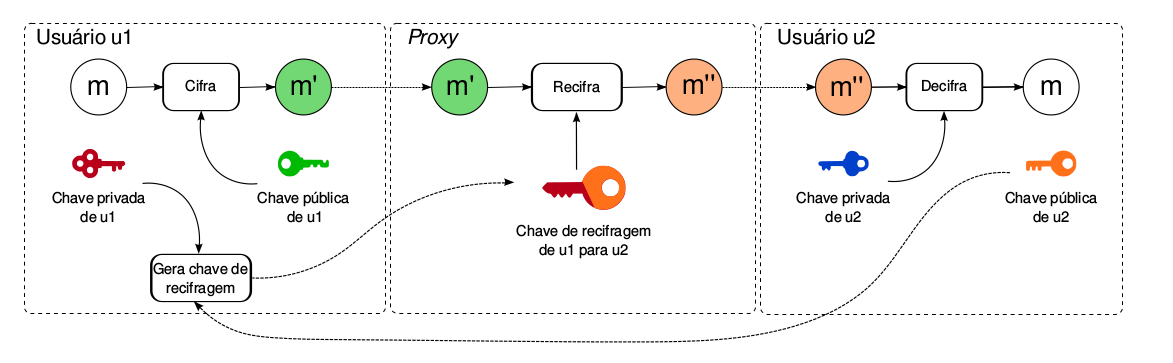
\includegraphics[width=17cm]{Figuras/recifragemPorProxy.png}
\caption{Recifragem por \emph{proxy} (\cite{mannes2016controle})} 
\label{figura:RecifragemProxy} 
\end{figure}

Há algumas premissas de operações padrão do esquemas de recifragem por \emph{proxy}. A implementação dos mesmos vai depender do tipo de recifragem[\cite{ateniese2006improved}, \cite{chow2010efficient}]:

\textbf{\textit{Configuração:}} Recebe como entrada um parâmetro de segurança $k$ e tem como saída uma tupla de parâmetros globais. 

\textbf{\textit{Geração de chaves:}} Gera os pares de chaves pública, $pk$, e privada, $sk$.

\textbf{\textit{Cifragem:}} Recebe $pk_{(u1)}$ e uma mensagem $m$, gera uma mensagem $\{m\}_{pk_{(u1)}}$.

\textbf{\textit{Geração de chave de recifragem:}} Tem como entrada a chave privada $sk_{(u1)}$ e a chave pública $pk_{(u2)}$ e como saída uma chave de recifragem $rk_{u1 \rightarrow u2}$.

\textbf{\textit{Recifragem:}} Recebe a chave de recifragem $rk_{u1 \rightarrow u2}$ e o texto cifrado $\{m\}_{pk_{(u1)}}$ , tem como saída $\{m\}_{pk_{(u2)}}$.

\textbf{\textit{Decifragem:}} Utilizando $sk_{(u2)}$ e $\{m\}_{pk_{(u2)}}$, gera como saída a mensagem $m$.

Afim de que o método seja considerado seguro foram incorporado diversas propriedades que respeitam 3 asserções básicas: (1) o \emph{proxy} não pode ser capaz de acessar o conteúdo da mensagem que recifra; (2) o usuário \emph{u}2 não pode obter o conteúdo da mensagem sem a interveção da função de recifragem; (3) O \emph{proxy} não pode, em hipótese nenhuma, obter as chaves privadas em posse das chave de recifragem e da mensagem cifrada[\cite{matsuo2007proxy},\cite{zhu2010new}].

Um resumo das possíveis caractéristicas de uma recifragem por \emph{proxy} está definido na tabela.

% ######## init table ########
%% ######## init table ########

\begin{table}[!htp]
\begin{tabular}{|c|c|c|}
\hline
Propriedades & Valores & Descrição \\ \hline
\multirow{Direção da delegação} & Unidirecional  & a  delegação $u1 \rightarrow u2$ não implica na delegação de $u2 \rightarrow u1$ \\ \cline{2-2}\cline{3-3} 
& Bidirecional  & a delegação u1 → u2 implica na delegação de u2 → u1 \\ \hline

\multirow{Número de saltos de recifragrem} & Único Salto \centering & somente mensagens originais podem ser recifradas \\ \cline{2-2}\cline{3-3} 
& Multiplos Saltos \centering & uma mensagem recifrada de u1 → u2 pode ser novamente recifrada de u2 → u3 \\ \hline

\multirow{Transitividade da chave de recifragem} & Transitivo & descrição transitivo \\ \cline{2-2}\cline{3-3} 
& Intransitivo \centering & o proxy não pode, a partir de rk u1→u2 e rk u2→u3 ,produzir rk u1→u3 \\ \hline

\multirow{Necessidade de iteração com o usuário} & Iterativo \centering & as chaves de recifragem são geradas por u1 com a necessidade de interações com u2 \\ \cline{2-2}\cline{3-3} 
& Não iterativo \centering & as chaves de recifragem são geradas por u1 sem a necessidade de interações com u2 \\ \hline

\multirow{Robustez contra conluio} & Robusto \centering & o usuário u2 e o proxy em conluio não conseguem recuperar a chave privada de u1 \\ \cline{2-2}\cline{3-3} 
& Não robusto \centering & o usuário u2 e o proxy em conluio conseguem recuperar a chave privada de u1 \\ \hline
\end{tabular}
\caption{Propriedades dos esquemas de recifragem por \textit{proxy}}
\label{table}
\end{table}

A recifragem por \emph{proxy} gerou então diversas abordagens com combinações mistas de propriedades. Dentro dessas abordagens está \emph{Efficient Unidirectional Proxy Re-Encryption} (EU-PRE) [\cite{chow2010efficient}] que contempla as seguintes propriedades: (1) \textit{Unirediconal}, (2) \textit{Único salto}, (3) \textit{Intrasitivo}, (4) \textit{Interativo} e (5) \textit{Robusto contra coluio}.

Outros duas abordagens também se encaixam nessas mesmas propriedades: são elas o esquema de \emph{proxy} invisível[\cite{jia2010cca}] e o esquema de \emph{proxy} anônimo [\cite{shao2012anonymous}]. Dessas três abordagens o EU-PRE se mostra mais simples e eficente, pois não implementa as funções de anonimato das mensagens cifradas e nem as funções de invisibilidade do \emph{proxy}.

Além disso, o trabalho de \cite{mannes2016controle} apresenta uma nova abordagem quanto ao EU-PRE. Retirando do sistema a necessidade de ter um agente de \emph{proxy}  sem impactar na segurança do processo.

Esse processo é feito através da otimização das equações matemáticas onde o processo de cifragem ainda ficará com o provedor de conteúdo e os de decifragem e recifragem ficarão a cargo do usuário. Eliminando assim um terceiro elemento do sistema, o que torna-o muito mais parecido com os que temos hoje.

% inclusão de apêndice
\section{Fundamentos}
\label{recifragem:fundamentos}
A recifragem por \emph{proxy} [\cite{blaze1998divertible}] é uma alternativa ao esquema criptográfico assimétrico tradicional [\cite{1363std}] que permite a delegação de direitos de acesso a messagens cifradas de maneira eficiente e mais segura. Em um cenário tradicional caso o usuário \emph{u}1 queira que somente os usuários \emph{u}2 e \emph{u}3 tenham acesso a suas mensagens cifradas ele primeiro cifra suas mensagens com sua chave privada (\emph{sk}1), em seguida cifra novamente com as chaves de \emph{u}2 e \emph{u}3 separadamente, de forma que ao distribuir essa mensagem cada um com suas respectivas chaves privadas e a chave pública de \emph{u}1 poderá decifrar a mensagem.

Em cenários onde se tem uma certa volatilidade quanto aos usuários e que a mensagem a ser transmitida não altera com tanta frequência, ou seja, existe mais mudanças de usuários que do conteúdo da mensagem. A abordagem tradicional de criptografia assimétrica se mostra uma abordagem pouco eficiente, visto que para cada vez que um usuário diferente necessitar consumir o conteúdo será necessário recifrar a mensagem a ser transmitida usando sua respectiva chave pública (\emph{pk}n) de forma que somente ele consiga reproduzi-la. Uma outra abordagem possível é através da entrega da chave privada de \emph{u}1 à \emph{u}n [\cite{ma2009group}]. Porém essa abodargem apresenta grande desvantagem visto que \emph{u}n terá acesso a chave privada de \emph{u}1 e por consequência terá acesso a todas as suas mensagens e por isso deve ser uma entidade confiável de \emph{u}1[\cite{libert2011unidirectional}].

A recifragem por \emph{proxy} explora as adptações do modelo tradicional introduzindo um novo elemento, o \emph{proxy}, que será responsável por intermediar a validação de chaves entre o usuário \emph{u}1 e seus consumidores. Simplificando é como se o \emph{proxy} agora fosse o responsável por fornecer as chaves de acesso ao conteúdo gerado por \emph{u}1 sem que o mesmo precise fornecer sua chave privada ou mesmo ter que recifrar todo o conteúdo com a chave pública dos usuários que irão consumir o mesmo.

Neste sistema o usuário \emph{u}1 irá cifrar seu conteúdo uma vez e o enviará para o \emph{proxy}. Paralelamente será gerado uma chave de recifragem que também será enviada ao \emph{proxy}. Dentro deste o conteúdo será recifrado utilizando agora a chave de recifragem de \emph{u}1 para \emph{u}n. Essa chave de recifragem permitirá ao usuário \emph{u}n decifrar o conteúdo recifrado pelo \emph{proxy} com a sua respectiva chave privada (\emph{pk}n) confome podemos observar na figura:
\begin{figure}[H]
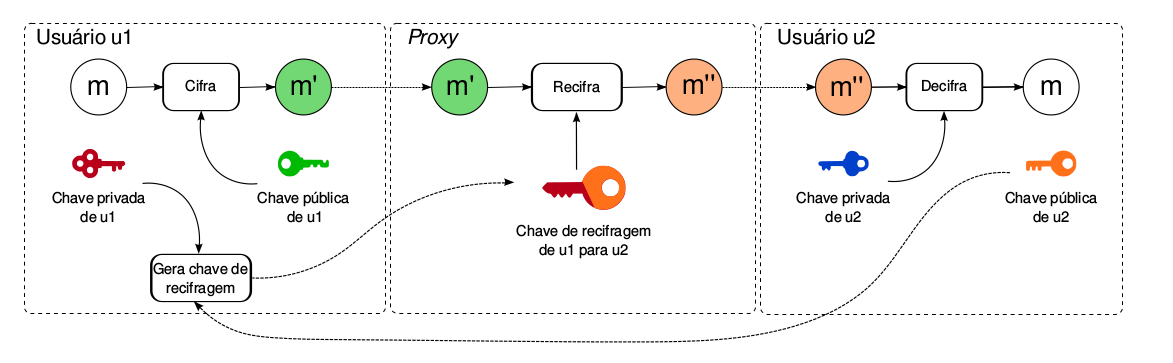
\includegraphics[width=17cm]{Figuras/recifragemPorProxy.png}
\caption{Recifragem por \emph{proxy} (\cite{mannes2016controle})} 
\label{figura:RecifragemProxy} 
\end{figure}

Há algumas premissas de operações padrão do esquemas de recifragem por \emph{proxy}. A implementação dos mesmos vai depender do tipo de recifragem[\cite{ateniese2006improved}, \cite{chow2010efficient}]:

\textbf{\textit{Configuração:}} Recebe como entrada um parâmetro de segurança $k$ e tem como saída uma tupla de parâmetros globais. 

\textbf{\textit{Geração de chaves:}} Gera os pares de chaves pública, $pk$, e privada, $sk$.

\textbf{\textit{Cifragem:}} Recebe $pk_{(u1)}$ e uma mensagem $m$, gera uma mensagem $\{m\}_{pk_{(u1)}}$.

\textbf{\textit{Geração de chave de recifragem:}} Tem como entrada a chave privada $sk_{(u1)}$ e a chave pública $pk_{(u2)}$ e como saída uma chave de recifragem $rk_{u1 \rightarrow u2}$.

\textbf{\textit{Recifragem:}} Recebe a chave de recifragem $rk_{u1 \rightarrow u2}$ e o texto cifrado $\{m\}_{pk_{(u1)}}$ , tem como saída $\{m\}_{pk_{(u2)}}$.

\textbf{\textit{Decifragem:}} Utilizando $sk_{(u2)}$ e $\{m\}_{pk_{(u2)}}$, gera como saída a mensagem $m$.

Afim de que o método seja considerado seguro foram incorporado diversas propriedades que respeitam 3 asserções básicas: (1) o \emph{proxy} não pode ser capaz de acessar o conteúdo da mensagem que recifra; (2) o usuário \emph{u}2 não pode obter o conteúdo da mensagem sem a interveção da função de recifragem; (3) O \emph{proxy} não pode, em hipótese nenhuma, obter as chaves privadas em posse das chave de recifragem e da mensagem cifrada[\cite{matsuo2007proxy},\cite{zhu2010new}].

Um resumo das possíveis caractéristicas de uma recifragem por \emph{proxy} está definido na tabela.

% ######## init table ########
%% ######## init table ########

\begin{table}[!htp]
\begin{tabular}{|c|c|c|}
\hline
Propriedades & Valores & Descrição \\ \hline
\multirow{Direção da delegação} & Unidirecional  & a  delegação $u1 \rightarrow u2$ não implica na delegação de $u2 \rightarrow u1$ \\ \cline{2-2}\cline{3-3} 
& Bidirecional  & a delegação u1 → u2 implica na delegação de u2 → u1 \\ \hline

\multirow{Número de saltos de recifragrem} & Único Salto \centering & somente mensagens originais podem ser recifradas \\ \cline{2-2}\cline{3-3} 
& Multiplos Saltos \centering & uma mensagem recifrada de u1 → u2 pode ser novamente recifrada de u2 → u3 \\ \hline

\multirow{Transitividade da chave de recifragem} & Transitivo & descrição transitivo \\ \cline{2-2}\cline{3-3} 
& Intransitivo \centering & o proxy não pode, a partir de rk u1→u2 e rk u2→u3 ,produzir rk u1→u3 \\ \hline

\multirow{Necessidade de iteração com o usuário} & Iterativo \centering & as chaves de recifragem são geradas por u1 com a necessidade de interações com u2 \\ \cline{2-2}\cline{3-3} 
& Não iterativo \centering & as chaves de recifragem são geradas por u1 sem a necessidade de interações com u2 \\ \hline

\multirow{Robustez contra conluio} & Robusto \centering & o usuário u2 e o proxy em conluio não conseguem recuperar a chave privada de u1 \\ \cline{2-2}\cline{3-3} 
& Não robusto \centering & o usuário u2 e o proxy em conluio conseguem recuperar a chave privada de u1 \\ \hline
\end{tabular}
\caption{Propriedades dos esquemas de recifragem por \textit{proxy}}
\label{table}
\end{table}

A recifragem por \emph{proxy} gerou então diversas abordagens com combinações mistas de propriedades. Dentro dessas abordagens está \emph{Efficient Unidirectional Proxy Re-Encryption} (EU-PRE) [\cite{chow2010efficient}] que contempla as seguintes propriedades: (1) \textit{Unirediconal}, (2) \textit{Único salto}, (3) \textit{Intrasitivo}, (4) \textit{Interativo} e (5) \textit{Robusto contra coluio}.

Outros duas abordagens também se encaixam nessas mesmas propriedades: são elas o esquema de \emph{proxy} invisível[\cite{jia2010cca}] e o esquema de \emph{proxy} anônimo [\cite{shao2012anonymous}]. Dessas três abordagens o EU-PRE se mostra mais simples e eficente, pois não implementa as funções de anonimato das mensagens cifradas e nem as funções de invisibilidade do \emph{proxy}.

Além disso, o trabalho de \cite{mannes2016controle} apresenta uma nova abordagem quanto ao EU-PRE. Retirando do sistema a necessidade de ter um agente de \emph{proxy}  sem impactar na segurança do processo.

Esse processo é feito através da otimização das equações matemáticas onde o processo de cifragem ainda ficará com o provedor de conteúdo e os de decifragem e recifragem ficarão a cargo do usuário. Eliminando assim um terceiro elemento do sistema, o que torna-o muito mais parecido com os que temos hoje.

%=====================================================

\end{document}

%=====================================================
